\documentclass{report}

%%%%%%%%%%%%%%%%%%%%%%%%%%%%%%%%%
% PACKAGE IMPORTS
%%%%%%%%%%%%%%%%%%%%%%%%%%%%%%%%%
\usepackage[tmargin=2cm,rmargin=1in,lmargin=1in,margin=0.85in,bmargin=2cm,footskip=.2in]{geometry}
\usepackage[none]{hyphenat}
\usepackage{amsmath,amsfonts,amsthm,amssymb,mathtools}
\allowdisplaybreaks
\usepackage{undertilde}
\usepackage{xfrac}
\usepackage[makeroom]{cancel}
\usepackage{mathtools}
\usepackage{bookmark}
\usepackage{enumitem}
\usepackage{kbordermatrix}
\renewcommand{\kbldelim}{(} % Change left delimiter to (
\renewcommand{\kbrdelim}{)} % Change right delimiter to )
\usepackage{hyperref,theoremref}
\hypersetup{
	pdftitle={Assignment},
	colorlinks=true, linkcolor=doc!90,
	bookmarksnumbered=true,
	bookmarksopen=true
}
\usepackage[most,many,breakable]{tcolorbox}
\usepackage{xcolor}
\usepackage{varwidth}
\usepackage{varwidth}
\usepackage{etoolbox}
%\usepackage{authblk}
\usepackage{nameref}
\usepackage{multicol,array}
\usepackage{tikz-cd}
\usepackage[ruled,vlined,linesnumbered]{algorithm2e}
\usepackage{comment} % enables the use of multi-line comments (\ifx \fi) 
\usepackage{import}
\usepackage{xifthen}
\usepackage{pdfpages}
\usepackage{svg}
\usepackage{transparent}
\usepackage{pgfplots}
\pgfplotsset{compat=1.18}
\usetikzlibrary{calc}
\usetikzlibrary{graphs}
\usetikzlibrary{graphs.standard}
% \usetikzlibrary{graphdrawing}

\newcommand\mycommfont[1]{\footnotesize\ttfamily\textcolor{blue}{#1}}
\SetCommentSty{mycommfont}
\newcommand{\incfig}[1]{%
    \def\svgwidth{\columnwidth}
    \import{./figures/}{#1.pdf_tex}
}


\usepackage{tikzsymbols}
% \renewcommand\qedsymbol{$\Laughey$}

\definecolor{commentgreen}{RGB}{2,112,10}
%%
%% Julia definition (c) 2014 Jubobs
%%
\lstdefinelanguage{Julia}%
  {morekeywords={abstract,break,case,catch,const,continue,do,else,elseif,%
      end,export,false,for,function,immutable,import,importall,if,in,%
      macro,module,otherwise,quote,return,switch,true,try,type,typealias,%
      using,while},%
   sensitive=true,%
   alsoother={$},%
   morecomment=[l]\#,%
   morecomment=[n]{\#=}{=\#},%
   morestring=[s]{"}{"},%
   morestring=[m]{'}{'},%
}[keywords,comments,strings]%

\lstset{%
    language        	= Julia,
    basicstyle      	= \ttfamily,
    keywordstyle    	= \bfseries\color{blue},
    stringstyle     	= \color{magenta},
    commentstyle    	= \color{commentgreen},
    showstringspaces	= false,
		numbers						= left,
		tabsize						= 4,
}

\definecolor{stringyellow}{RGB}{227, 78, 48}
%% 
%% Shamelessly stolen from Vivi on Stackoverflow
%% https://tex.stackexchange.com/questions/75116/what-can-i-use-to-typeset-matlab-code-in-my-document
%%
\lstset{language=Matlab,%
    %basicstyle=\color{red},
    breaklines=true,%
    morekeywords={matlab2tikz},
		morekeywords={subtitle}
    keywordstyle=\color{blue},%
    morekeywords=[2]{1}, keywordstyle=[2]{\color{black}},
    identifierstyle=\color{black},%
    stringstyle=\color{stringyellow},
    commentstyle=\color{commentgreen},%
    showstringspaces=false,%without this there will be a symbol in the places where there is a space
    numbers=left,%
		firstnumber=1,
    % numberstyle={\tiny \color{black}},% size of the numbers
    % numbersep=9pt, % this defines how far the numbers are from the text
    emph=[1]{for,end,break},emphstyle=[1]\color{red}, %some words to emphasise
    %emph=[2]{word1,word2}, emphstyle=[2]{style},    
}

%% 
%% Shamelessly stolen from egreg on Stackoverflow
%% https://tex.stackexchange.com/questions/280681/how-to-have-multiple-lines-of-intertext-within-align-environment
%%
\newlength{\normalparindent}
\AtBeginDocument{\setlength{\normalparindent}{\parindent}}
\newcommand{\longintertext}[1]{%
  \intertext{%
    \parbox{\linewidth}{%
      \setlength{\parindent}{\normalparindent}
      \noindent#1%
    }%
  }%
}

%\usepackage{import}
%\usepackage{xifthen}
%\usepackage{pdfpages}
%\usepackage{transparent}

%%%%%%%%%%%%%%%%%%%%%%%%%%%%%%
% SELF MADE COLORS
%%%%%%%%%%%%%%%%%%%%%%%%%%%%%%
\definecolor{myg}{RGB}{56, 140, 70}
\definecolor{myb}{RGB}{45, 111, 177}
\definecolor{myr}{RGB}{199, 68, 64}
\definecolor{mytheorembg}{HTML}{F2F2F9}
\definecolor{mytheoremfr}{HTML}{00007B}
\definecolor{mylenmabg}{HTML}{FFFAF8}
\definecolor{mylenmafr}{HTML}{983b0f}
\definecolor{mypropbg}{HTML}{f2fbfc}
\definecolor{mypropfr}{HTML}{191971}
\definecolor{myexamplebg}{HTML}{F2FBF8}
\definecolor{myexamplefr}{HTML}{88D6D1}
\definecolor{myexampleti}{HTML}{2A7F7F}
\definecolor{mydefinitbg}{HTML}{E5E5FF}
\definecolor{mydefinitfr}{HTML}{3F3FA3}
\definecolor{notesgreen}{RGB}{0,162,0}
\definecolor{myp}{RGB}{197, 92, 212}
\definecolor{mygr}{HTML}{2C3338}
\definecolor{myred}{RGB}{127,0,0}
\definecolor{myyellow}{RGB}{169,121,69}
\definecolor{myexercisebg}{HTML}{F2FBF8}
\definecolor{myexercisefg}{HTML}{88D6D1}

%%%%%%%%%%%%%%%%%%%%%%%%%%%%
% TCOLORBOX SETUPS
%%%%%%%%%%%%%%%%%%%%%%%%%%%%
\setlength{\parindent}{0pt}

%================================
% THEOREM BOX
%================================
\tcbuselibrary{theorems,skins,hooks}
\newtcbtheorem[number within=section]{Theorem}{Theorem}
{%
	enhanced,
	breakable,
	colback = mytheorembg,
	frame hidden,
	boxrule = 0sp,
	borderline west = {2pt}{0pt}{mytheoremfr},
	sharp corners,
	detach title,
	before upper = \tcbtitle\par\smallskip,
	coltitle = mytheoremfr,
	fonttitle = \bfseries\sffamily,
	description font = \mdseries,
	separator sign none,
	segmentation style={solid, mytheoremfr},
}
{th}

\tcbuselibrary{theorems,skins,hooks}
\newtcbtheorem[number within=chapter]{theorem}{Theorem}
{%
	enhanced,
	breakable,
	colback = mytheorembg,
	frame hidden,
	boxrule = 0sp,
	borderline west = {2pt}{0pt}{mytheoremfr},
	sharp corners,
	detach title,
	before upper = \tcbtitle\par\smallskip,
	coltitle = mytheoremfr,
	fonttitle = \bfseries\sffamily,
	description font = \mdseries,
	separator sign none,
	segmentation style={solid, mytheoremfr},
}
{th}


\tcbuselibrary{theorems,skins,hooks}
\newtcolorbox{Theoremcon}
{%
	enhanced
	,breakable
	,colback = mytheorembg
	,frame hidden
	,boxrule = 0sp
	,borderline west = {2pt}{0pt}{mytheoremfr}
	,sharp corners
	,description font = \mdseries
	,separator sign none
}

%================================
% Corollery
%================================
\tcbuselibrary{theorems,skins,hooks}
\newtcbtheorem[number within=section]{Corollary}{Corollary}
{%
	enhanced
	,breakable
	,colback = myp!10
	,frame hidden
	,boxrule = 0sp
	,borderline west = {2pt}{0pt}{myp!85!black}
	,sharp corners
	,detach title
	,before upper = \tcbtitle\par\smallskip
	,coltitle = myp!85!black
	,fonttitle = \bfseries\sffamily
	,description font = \mdseries
	,separator sign none
	,segmentation style={solid, myp!85!black}
}
{th}
\tcbuselibrary{theorems,skins,hooks}
\newtcbtheorem[number within=chapter]{corollary}{Corollary}
{%
	enhanced
	,breakable
	,colback = myp!10
	,frame hidden
	,boxrule = 0sp
	,borderline west = {2pt}{0pt}{myp!85!black}
	,sharp corners
	,detach title
	,before upper = \tcbtitle\par\smallskip
	,coltitle = myp!85!black
	,fonttitle = \bfseries\sffamily
	,description font = \mdseries
	,separator sign none
	,segmentation style={solid, myp!85!black}
}
{th}

%================================
% LENMA
%================================
\tcbuselibrary{theorems,skins,hooks}
\newtcbtheorem[number within=section]{Lenma}{Lenma}
{%
	enhanced,
	breakable,
	colback = mylenmabg,
	frame hidden,
	boxrule = 0sp,
	borderline west = {2pt}{0pt}{mylenmafr},
	sharp corners,
	detach title,
	before upper = \tcbtitle\par\smallskip,
	coltitle = mylenmafr,
	fonttitle = \bfseries\sffamily,
	description font = \mdseries,
	separator sign none,
	segmentation style={solid, mylenmafr},
}
{th}

\tcbuselibrary{theorems,skins,hooks}
\newtcbtheorem[number within=chapter]{lenma}{Lenma}
{%
	enhanced,
	breakable,
	colback = mylenmabg,
	frame hidden,
	boxrule = 0sp,
	borderline west = {2pt}{0pt}{mylenmafr},
	sharp corners,
	detach title,
	before upper = \tcbtitle\par\smallskip,
	coltitle = mylenmafr,
	fonttitle = \bfseries\sffamily,
	description font = \mdseries,
	separator sign none,
	segmentation style={solid, mylenmafr},
}
{th}

%================================
% PROPOSITION
%================================
\tcbuselibrary{theorems,skins,hooks}
\newtcbtheorem[number within=section]{Prop}{Proposition}
{%
	enhanced,
	breakable,
	colback = mypropbg,
	frame hidden,
	boxrule = 0sp,
	borderline west = {2pt}{0pt}{mypropfr},
	sharp corners,
	detach title,
	before upper = \tcbtitle\par\smallskip,
	coltitle = mypropfr,
	fonttitle = \bfseries\sffamily,
	description font = \mdseries,
	separator sign none,
	segmentation style={solid, mypropfr},
}
{th}

\tcbuselibrary{theorems,skins,hooks}
\newtcbtheorem[number within=chapter]{prop}{Proposition}
{%
	enhanced,
	breakable,
	colback = mypropbg,
	frame hidden,
	boxrule = 0sp,
	borderline west = {2pt}{0pt}{mypropfr},
	sharp corners,
	detach title,
	before upper = \tcbtitle\par\smallskip,
	coltitle = mypropfr,
	fonttitle = \bfseries\sffamily,
	description font = \mdseries,
	separator sign none,
	segmentation style={solid, mypropfr},
}
{th}

%================================
% CLAIM
%================================
\tcbuselibrary{theorems,skins,hooks}
\newtcbtheorem[number within=section]{claim}{Claim}
{%
	enhanced
	,breakable
	,colback = myg!10
	,frame hidden
	,boxrule = 0sp
	,borderline west = {2pt}{0pt}{myg}
	,sharp corners
	,detach title
	,before upper = \tcbtitle\par\smallskip
	,coltitle = myg!85!black
	,fonttitle = \bfseries\sffamily
	,description font = \mdseries
	,separator sign none
	,segmentation style={solid, myg!85!black}
}
{th}

%================================
% Exercise
%================================
\tcbuselibrary{theorems,skins,hooks}
\newtcbtheorem[number within=section]{Exercise}{Exercise}
{%
	enhanced,
	breakable,
	colback = myexercisebg,
	frame hidden,
	boxrule = 0sp,
	borderline west = {2pt}{0pt}{myexercisefg},
	sharp corners,
	detach title,
	before upper = \tcbtitle\par\smallskip,
	coltitle = myexercisefg,
	fonttitle = \bfseries\sffamily,
	description font = \mdseries,
	separator sign none,
	segmentation style={solid, myexercisefg},
}
{th}

\tcbuselibrary{theorems,skins,hooks}
\newtcbtheorem[number within=chapter]{exercise}{Exercise}
{%
	enhanced,
	breakable,
	colback = myexercisebg,
	frame hidden,
	boxrule = 0sp,
	borderline west = {2pt}{0pt}{myexercisefg},
	sharp corners,
	detach title,
	before upper = \tcbtitle\par\smallskip,
	coltitle = myexercisefg,
	fonttitle = \bfseries\sffamily,
	description font = \mdseries,
	separator sign none,
	segmentation style={solid, myexercisefg},
}
{th}

%================================
% EXAMPLE BOX
%================================
\newtcbtheorem[number within=section]{Example}{Example}
{%
	colback = myexamplebg
	,breakable
	,colframe = myexamplefr
	,coltitle = myexampleti
	,boxrule = 1pt
	,sharp corners
	,detach title
	,before upper=\tcbtitle\par\smallskip
	,fonttitle = \bfseries
	,description font = \mdseries
	,separator sign none
	,description delimiters parenthesis
}
{ex}

\newtcbtheorem[number within=chapter]{example}{Example}
{%
	colback = myexamplebg
	,breakable
	,colframe = myexamplefr
	,coltitle = myexampleti
	,boxrule = 1pt
	,sharp corners
	,detach title
	,before upper=\tcbtitle\par\smallskip
	,fonttitle = \bfseries
	,description font = \mdseries
	,separator sign none
	,description delimiters parenthesis
}
{ex}

%================================
% DEFINITION BOX
%================================
\newtcbtheorem[number within=section]{Definition}{Definition}{enhanced,
	before skip=2mm,after skip=2mm, colback=red!5,colframe=red!80!black,boxrule=0.5mm,
	attach boxed title to top left={xshift=1cm,yshift*=1mm-\tcboxedtitleheight}, varwidth boxed title*=-3cm,
	boxed title style={frame code={
					\path[fill=tcbcolback]
					([yshift=-1mm,xshift=-1mm]frame.north west)
					arc[start angle=0,end angle=180,radius=1mm]
					([yshift=-1mm,xshift=1mm]frame.north east)
					arc[start angle=180,end angle=0,radius=1mm];
					\path[left color=tcbcolback!60!black,right color=tcbcolback!60!black,
						middle color=tcbcolback!80!black]
					([xshift=-2mm]frame.north west) -- ([xshift=2mm]frame.north east)
					[rounded corners=1mm]-- ([xshift=1mm,yshift=-1mm]frame.north east)
					-- (frame.south east) -- (frame.south west)
					-- ([xshift=-1mm,yshift=-1mm]frame.north west)
					[sharp corners]-- cycle;
				},interior engine=empty,
		},
	fonttitle=\bfseries,
	title={#2},#1}{def}
\newtcbtheorem[number within=chapter]{definition}{Definition}{enhanced,
	before skip=2mm,after skip=2mm, colback=red!5,colframe=red!80!black,boxrule=0.5mm,
	attach boxed title to top left={xshift=1cm,yshift*=1mm-\tcboxedtitleheight}, varwidth boxed title*=-3cm,
	boxed title style={frame code={
					\path[fill=tcbcolback]
					([yshift=-1mm,xshift=-1mm]frame.north west)
					arc[start angle=0,end angle=180,radius=1mm]
					([yshift=-1mm,xshift=1mm]frame.north east)
					arc[start angle=180,end angle=0,radius=1mm];
					\path[left color=tcbcolback!60!black,right color=tcbcolback!60!black,
						middle color=tcbcolback!80!black]
					([xshift=-2mm]frame.north west) -- ([xshift=2mm]frame.north east)
					[rounded corners=1mm]-- ([xshift=1mm,yshift=-1mm]frame.north east)
					-- (frame.south east) -- (frame.south west)
					-- ([xshift=-1mm,yshift=-1mm]frame.north west)
					[sharp corners]-- cycle;
				},interior engine=empty,
		},
	fonttitle=\bfseries,
	title={#2},#1}{def}

%================================
% Solution BOX
%================================
\makeatletter
\newtcbtheorem{question}{Question}{enhanced,
	breakable,
	colback=white,
	colframe=myb!80!black,
	attach boxed title to top left={yshift*=-\tcboxedtitleheight},
	fonttitle=\bfseries,
	title={#2},
	boxed title size=title,
	boxed title style={%
			sharp corners,
			rounded corners=northwest,
			colback=tcbcolframe,
			boxrule=0pt,
		},
	underlay boxed title={%
			\path[fill=tcbcolframe] (title.south west)--(title.south east)
			to[out=0, in=180] ([xshift=5mm]title.east)--
			(title.center-|frame.east)
			[rounded corners=\kvtcb@arc] |-
			(frame.north) -| cycle;
		},
	#1
}{def}
\makeatother

%================================
% SOLUTION BOX
%================================
\makeatletter
\newtcolorbox{solution}{enhanced,
	breakable,
	colback=white,
	colframe=myg!80!black,
	attach boxed title to top left={yshift*=-\tcboxedtitleheight},
	title=Solution,
	boxed title size=title,
	boxed title style={%
			sharp corners,
			rounded corners=northwest,
			colback=tcbcolframe,
			boxrule=0pt,
		},
	underlay boxed title={%
			\path[fill=tcbcolframe] (title.south west)--(title.south east)
			to[out=0, in=180] ([xshift=5mm]title.east)--
			(title.center-|frame.east)
			[rounded corners=\kvtcb@arc] |-
			(frame.north) -| cycle;
		},
}
\makeatother

%================================
% Question BOX
%================================
\makeatletter
\newtcbtheorem{qstion}{Question}{enhanced,
	breakable,
	colback=white,
	colframe=mygr,
	attach boxed title to top left={yshift*=-\tcboxedtitleheight},
	fonttitle=\bfseries,
	title={#2},
	boxed title size=title,
	boxed title style={%
			sharp corners,
			rounded corners=northwest,
			colback=tcbcolframe,
			boxrule=0pt,
		},
	underlay boxed title={%
			\path[fill=tcbcolframe] (title.south west)--(title.south east)
			to[out=0, in=180] ([xshift=5mm]title.east)--
			(title.center-|frame.east)
			[rounded corners=\kvtcb@arc] |-
			(frame.north) -| cycle;
		},
	#1
}{def}
\makeatother

\newtcbtheorem[number within=chapter]{wconc}{Wrong Concept}{
	breakable,
	enhanced,
	colback=white,
	colframe=myr,
	arc=0pt,
	outer arc=0pt,
	fonttitle=\bfseries\sffamily\large,
	colbacktitle=myr,
	attach boxed title to top left={},
	boxed title style={
			enhanced,
			skin=enhancedfirst jigsaw,
			arc=3pt,
			bottom=0pt,
			interior style={fill=myr}
		},
	#1
}{def}

%================================
% NOTE BOX
%================================
\usetikzlibrary{arrows,calc,shadows.blur}
\tcbuselibrary{skins}
\newtcolorbox{note}[1][]{%
	enhanced jigsaw,
	colback=gray!20!white,%
	colframe=gray!80!black,
	size=small,
	boxrule=1pt,
	title=\textbf{Note:-},
	halign title=flush center,
	coltitle=black,
	breakable,
	drop shadow=black!50!white,
	attach boxed title to top left={xshift=1cm,yshift=-\tcboxedtitleheight/2,yshifttext=-\tcboxedtitleheight/2},
	minipage boxed title=1.5cm,
	boxed title style={%
			colback=white,
			size=fbox,
			boxrule=1pt,
			boxsep=2pt,
			underlay={%
					\coordinate (dotA) at ($(interior.west) + (-0.5pt,0)$);
					\coordinate (dotB) at ($(interior.east) + (0.5pt,0)$);
					\begin{scope}
						\clip (interior.north west) rectangle ([xshift=3ex]interior.east);
						\filldraw [white, blur shadow={shadow opacity=60, shadow yshift=-.75ex}, rounded corners=2pt] (interior.north west) rectangle (interior.south east);
					\end{scope}
					\begin{scope}[gray!80!black]
						\fill (dotA) circle (2pt);
						\fill (dotB) circle (2pt);
					\end{scope}
				},
		},
	#1,
}

%%%%%%%%%%%%%%%%%%%%%%%%%%%%%%
% SELF MADE COMMANDS
%%%%%%%%%%%%%%%%%%%%%%%%%%%%%%
\newcommand{\thm}[2]{\begin{Theorem}{#1}{}#2\end{Theorem}}
\newcommand{\cor}[2]{\begin{Corollary}{#1}{}#2\end{Corollary}}
\newcommand{\mlenma}[2]{\begin{Lenma}{#1}{}#2\end{Lenma}}
\newcommand{\mprop}[2]{\begin{Prop}{#1}{}#2\end{Prop}}
\newcommand{\clm}[3]{\begin{claim}{#1}{#2}#3\end{claim}}
\newcommand{\wc}[2]{\begin{wconc}{#1}{}\setlength{\parindent}{1cm}#2\end{wconc}}
\newcommand{\thmcon}[1]{\begin{Theoremcon}{#1}\end{Theoremcon}}
\newcommand{\ex}[2]{\begin{Example}{#1}{}#2\end{Example}}
\newcommand{\dfn}[2]{\begin{Definition}[colbacktitle=red!75!black]{#1}{}#2\end{Definition}}
\newcommand{\dfnc}[2]{\begin{definition}[colbacktitle=red!75!black]{#1}{}#2\end{definition}}
\newcommand{\qs}[2]{\begin{question}{#1}{}#2\end{question}}
\newcommand{\pf}[2]{\begin{myproof}[#1]#2\end{myproof}}
\newcommand{\nt}[1]{\begin{note}#1\end{note}}

\newcommand*\circled[1]{\tikz[baseline=(char.base)]{
		\node[shape=circle,draw,inner sep=1pt] (char) {#1};}}
\newcommand\getcurrentref[1]{%
	\ifnumequal{\value{#1}}{0}
	{??}
	{\the\value{#1}}%
}
\newcommand{\getCurrentSectionNumber}{\getcurrentref{section}}
\newenvironment{myproof}[1][\proofname]{%
	\proof[\bfseries #1: ]%
}{\endproof}

\newcommand{\mclm}[2]{\begin{myclaim}[#1]#2\end{myclaim}}
\newenvironment{myclaim}[1][\claimname]{\proof[\bfseries #1: ]}{}

\newcounter{mylabelcounter}

\makeatletter
\newcommand{\setword}[2]{%
	\phantomsection
	#1\def\@currentlabel{\unexpanded{#1}}\label{#2}%
}
\makeatother

\tikzset{
	symbol/.style={
			draw=none,
			every to/.append style={
					edge node={node [sloped, allow upside down, auto=false]{$#1$}}}
		}
}

% deliminators
\DeclarePairedDelimiter{\abs}{\lvert}{\rvert}
\DeclarePairedDelimiter{\norm}{\lVert}{\rVert}

\DeclarePairedDelimiter{\ceil}{\lceil}{\rceil}
\DeclarePairedDelimiter{\floor}{\lfloor}{\rfloor}
\DeclarePairedDelimiter{\round}{\lfloor}{\rceil}

\newsavebox\diffdbox
\newcommand{\slantedromand}{{\mathpalette\makesl{d}}}
\newcommand{\makesl}[2]{%
\begingroup
\sbox{\diffdbox}{$\mathsurround=0pt#1\mathrm{#2}$}%
\pdfsave
\pdfsetmatrix{1 0 0.2 1}%
\rlap{\usebox{\diffdbox}}%
\pdfrestore
\hskip\wd\diffdbox
\endgroup
}
\newcommand{\dd}[1][]{\ensuremath{\mathop{}\!\ifstrempty{#1}{%
\slantedromand\@ifnextchar^{\hspace{0.2ex}}{\hspace{0.1ex}}}%
{\slantedromand\hspace{0.2ex}^{#1}}}}
\ProvideDocumentCommand\dv{o m g}{%
  \ensuremath{%
    \IfValueTF{#3}{%
      \IfNoValueTF{#1}{%
        \frac{\dd #2}{\dd #3}%
      }{%
        \frac{\dd^{#1} #2}{\dd #3^{#1}}%
      }%
    }{%
      \IfNoValueTF{#1}{%
        \frac{\dd}{\dd #2}%
      }{%
        \frac{\dd^{#1}}{\dd #2^{#1}}%
      }%
    }%
  }%
}
\providecommand*{\pdv}[3][]{\frac{\partial^{#1}#2}{\partial#3^{#1}}}
%  - others
\DeclareMathOperator{\Lap}{\mathcal{L}}
\DeclareMathOperator{\Var}{Var} % varience
\DeclareMathOperator{\Cov}{Cov} % covarience
\DeclareMathOperator{\E}{E} % expected

% Since the amsthm package isn't loaded

% I dot not prefer the slanted \leq ;P
% % I prefer the slanted \leq
% \let\oldleq\leq % save them in case they're every wanted
% \let\oldgeq\geq
% \renewcommand{\leq}{\leqslant}
% \renewcommand{\geq}{\geqslant}

% % redefine matrix env to allow for alignment, use r as default
% \renewcommand*\env@matrix[1][r]{\hskip -\arraycolsep
%     \let\@ifnextchar\new@ifnextchar
%     \array{*\c@MaxMatrixCols #1}}

%\usepackage{framed}
%\usepackage{titletoc}
%\usepackage{etoolbox}
%\usepackage{lmodern}

%\patchcmd{\tableofcontents}{\contentsname}{\sffamily\contentsname}{}{}

%\renewenvironment{leftbar}
%{\def\FrameCommand{\hspace{6em}%
%		{\color{myyellow}\vrule width 2pt depth 6pt}\hspace{1em}}%
%	\MakeFramed{\parshape 1 0cm \dimexpr\textwidth-6em\relax\FrameRestore}\vskip2pt%
%}
%{\endMakeFramed}

%\titlecontents{chapter}
%[0em]{\vspace*{2\baselineskip}}
%{\parbox{4.5em}{%
%		\hfill\Huge\sffamily\bfseries\color{myred}\thecontentspage}%
%	\vspace*{-2.3\baselineskip}\leftbar\textsc{\small\chaptername~\thecontentslabel}\\\sffamily}
%{}{\endleftbar}
%\titlecontents{section}
%[8.4em]
%{\sffamily\contentslabel{3em}}{}{}
%{\hspace{0.5em}\nobreak\itshape\color{myred}\contentspage}
%\titlecontents{subsection}
%[8.4em]
%{\sffamily\contentslabel{3em}}{}{}  
%{\hspace{0.5em}\nobreak\itshape\color{myred}\contentspage}

%%%%%%%%%%%%%%%%%%%%%%%%%%%%%%%%%%%%%%%%%%%
% TABLE OF CONTENTS
%%%%%%%%%%%%%%%%%%%%%%%%%%%%%%%%%%%%%%%%%%%
\usepackage{tikz}
\definecolor{doc}{RGB}{0,60,110}
\usepackage{titletoc}
\contentsmargin{0cm}
\titlecontents{chapter}[3.7pc]
{\addvspace{30pt}%
	\begin{tikzpicture}[remember picture, overlay]%
		\draw[fill=doc!60,draw=doc!60] (-7,-.1) rectangle (-0.9,.5);%
		\pgftext[left,x=-3.5cm,y=0.2cm]{\color{white}\Large\sc\bfseries Chapter\ \thecontentslabel};%
	\end{tikzpicture}\color{doc!60}\large\sc\bfseries}%
{}
{}
{\;\titlerule\;\large\sc\bfseries Page \thecontentspage
	\begin{tikzpicture}[remember picture, overlay]
		\draw[fill=doc!60,draw=doc!60] (2pt,0) rectangle (4,0.1pt);
	\end{tikzpicture}}%
\titlecontents{section}[3.7pc]
{\addvspace{2pt}}
{\contentslabel[\thecontentslabel]{2pc}}
{}
{\hfill\small \thecontentspage}
[]
\titlecontents*{subsection}[3.7pc]
{\addvspace{-1pt}\small}
{}
{}
{\ --- \small\thecontentspage}
[ \textbullet\ ][]

\makeatletter
\renewcommand{\tableofcontents}{%
	\chapter*{%
	  \vspace*{-20\p@}%
	  \begin{tikzpicture}[remember picture, overlay]%
		  \pgftext[right,x=15cm,y=0.2cm]{\color{doc!60}\Huge\sc\bfseries \contentsname};%
		  \draw[fill=doc!60,draw=doc!60] (13,-.75) rectangle (20,1);%
		  \clip (13,-.75) rectangle (20,1);
		  \pgftext[right,x=15cm,y=0.2cm]{\color{white}\Huge\sc\bfseries \contentsname};%
	  \end{tikzpicture}}%
	\@starttoc{toc}}
\makeatother

\newcommand{\inv}{^{-1}}
\newcommand{\opname}{\operatorname}
\newcommand{\surjto}{\twoheadrightarrow}
% \newcommand{\injto}{\hookrightarrow}
\newcommand{\injto}{\rightarrowtail}
\newcommand{\bijto}{\leftrightarrow}

\newcommand{\liff}{\leftrightarrow}
\newcommand{\notliff}{\mathrel{\ooalign{$\leftrightarrow$\cr\hidewidth$/$\hidewidth}}}
\newcommand{\lthen}{\rightarrow}
\let\varlnot\lnot
\newcommand{\ordsim}{\mathord{\sim}}
\renewcommand{\lnot}{\ordsim}
\newcommand{\lxor}{\oplus}
\newcommand{\lnand}{\barwedge}
\newcommand{\divs}{\mathrel{\mid}}
\newcommand{\ndivs}{\mathrel{\nmid}}
\def\contra{\tikz[baseline, x=0.22em, y=0.22em, line width=0.032em]\draw (0,2.83)--(2.83,0) (0.71,3.54)--(3.54,0.71) (0,0.71)--(2.83,3.54) (0.71,0)--(3.54,2.83);}

\newcommand{\On}{\mathrm{On}} % ordinals
\DeclareMathOperator{\img}{im} % Image
\DeclareMathOperator{\Img}{Im} % Image
\DeclareMathOperator{\coker}{coker} % Cokernel
\DeclareMathOperator{\Coker}{Coker} % Cokernel
\DeclareMathOperator{\Ker}{Ker} % Kernel
\DeclareMathOperator{\rank}{rank}
\DeclareMathOperator{\Spec}{Spec} % spectrum
\DeclareMathOperator{\Tr}{Tr} % trace
\DeclareMathOperator{\pr}{pr} % projection
\DeclareMathOperator{\ext}{ext} % extension
\DeclareMathOperator{\pred}{pred} % predecessor
\DeclareMathOperator{\dom}{dom} % domain
\DeclareMathOperator{\ran}{ran} % range
\DeclareMathOperator{\Hom}{Hom} % homomorphism
\DeclareMathOperator{\Mor}{Mor} % morphisms
\DeclareMathOperator{\End}{End} % endomorphism
\DeclareMathOperator{\Span}{span}
\newcommand{\Mod}{\mathbin{\mathrm{mod}}}

\newcommand{\eps}{\epsilon}
\newcommand{\veps}{\varepsilon}
\newcommand{\ol}{\overline}
\newcommand{\ul}{\underline}
\newcommand{\wt}{\widetilde}
\newcommand{\wh}{\widehat}
\newcommand{\ut}{\utilde}
\newcommand{\unit}[1]{\ut{\hat{#1}}}
\newcommand{\emp}{\varnothing}

\newcommand{\vocab}[1]{\textbf{\color{blue} #1}}
\providecommand{\half}{\frac{1}{2}}
\newcommand{\dang}{\measuredangle} %% Directed angle
\newcommand{\ray}[1]{\overrightarrow{#1}}
\newcommand{\seg}[1]{\overline{#1}}
\newcommand{\arc}[1]{\wideparen{#1}}
\DeclareMathOperator{\cis}{cis}
\DeclareMathOperator*{\lcm}{lcm}
\DeclareMathOperator*{\argmin}{arg min}
\DeclareMathOperator*{\argmax}{arg max}
\newcommand{\cycsum}{\sum_{\mathrm{cyc}}}
\newcommand{\symsum}{\sum_{\mathrm{sym}}}
\newcommand{\cycprod}{\prod_{\mathrm{cyc}}}
\newcommand{\symprod}{\prod_{\mathrm{sym}}}
\newcommand{\parinn}{\setlength{\parindent}{1cm}}
\newcommand{\parinf}{\setlength{\parindent}{0cm}}
% \newcommand{\norm}{\|\cdot\|}
\newcommand{\inorm}{\norm_{\infty}}
\newcommand{\opensets}{\{V_{\alpha}\}_{\alpha\in I}}
\newcommand{\oset}{V_{\alpha}}
\newcommand{\opset}[1]{V_{\alpha_{#1}}}
\newcommand{\lub}{\text{lub}}
\newcommand{\lm}{\lambda}
\newcommand{\uin}{\mathbin{\rotatebox[origin=c]{90}{$\in$}}}
\newcommand{\usubset}{\mathbin{\rotatebox[origin=c]{90}{$\subset$}}}
\newcommand{\lt}{\left}
\newcommand{\rt}{\right}
\newcommand{\bs}[1]{\boldsymbol{#1}}
\newcommand{\exs}{\exists}
\newcommand{\st}{\strut}
\newcommand{\dps}[1]{\displaystyle{#1}}

\newcommand{\sol}{\textbf{\textit{Solution:}} }
\newcommand{\solve}[1]{\textbf{\textit{Solution: }} #1 \qed}
% \newcommand{\proof}{\underline{\textit{proof:}}\\}

\DeclareMathOperator{\sech}{sech}
\DeclareMathOperator{\csch}{csch}
\DeclareMathOperator{\arcsec}{arcsec}
\DeclareMathOperator{\arccsc}{arccsc}
\DeclareMathOperator{\arccot}{arccot}
\DeclareMathOperator{\arsinh}{arsinh}
\DeclareMathOperator{\arcosh}{arcosh}
\DeclareMathOperator{\artanh}{artanh}
\DeclareMathOperator{\arcsch}{arcsch}
\DeclareMathOperator{\arsech}{arsech}
\DeclareMathOperator{\arcoth}{arcoth}

\newcommand{\sinx}{\sin x}          \newcommand{\arcsinx}{\arcsin x}    
\newcommand{\cosx}{\cos x}          \newcommand{\arccosx}{\arccosx}
\newcommand{\tanx}{\tan x}          \newcommand{\arctanx}{\arctan x}
\newcommand{\cscx}{\csc x}          \newcommand{\arccscx}{\arccsc x}
\newcommand{\secx}{\sec x}          \newcommand{\arcsecx}{\arcsec x}
\newcommand{\cotx}{\cot x}          \newcommand{\arccotx}{\arccot x}
\newcommand{\sinhx}{\sinh x}          \newcommand{\arsinhx}{\arsinh x}
\newcommand{\coshx}{\cosh x}          \newcommand{\arcoshx}{\arcosh x}
\newcommand{\tanhx}{\tanh x}          \newcommand{\artanhx}{\artanh x}
\newcommand{\cschx}{\csch x}          \newcommand{\arcschx}{\arcsch x}
\newcommand{\sechx}{\sech x}          \newcommand{\arsechx}{\arsech x}
\newcommand{\cothx}{\coth x}          \newcommand{\arcothx}{\arcoth x}
\newcommand{\lnx}{\ln x}
\newcommand{\expx}{\exp x}

\newcommand{\Theom}{\textbf{Theorem. }}
\newcommand{\Lemma}{\textbf{Lemma. }}
\newcommand{\Corol}{\textbf{Corollary. }}
\newcommand{\Remar}{\textit{Remark. }}
\newcommand{\Defin}[1]{\textbf{Definition} (#1).}
\newcommand{\Claim}{\textbf{Claim. }}
\newcommand{\Propo}{\textbf{Proposition. }}

\newcommand{\lb}{\left(}
\newcommand{\rb}{\right)}
\newcommand{\lbr}{\left\lbrace}
\newcommand{\rbr}{\right\rbrace}
\newcommand{\lsb}{\left[}
\newcommand{\rsb}{\right]}
\newcommand{\bracks}[1]{\lb #1 \rb}
\newcommand{\braces}[1]{\lbr #1 \rbr}
\newcommand{\suchthat}{\medspace\middle|\medspace}
\newcommand{\sqbracks}[1]{\lsb #1 \rsb}
\renewcommand{\abs}[1]{\left| #1 \right|}
\newcommand{\Mag}[1]{\left|\left| #1 \right|\right|}
\renewcommand{\floor}[1]{\left\lfloor #1 \right\rfloor}
\renewcommand{\ceil}[1]{\left\lceil #1 \right\rceil}

\newcommand{\cd}{\cdot}
\newcommand{\tf}{\therefore}
\newcommand{\Let}{\text{Let }}
\newcommand{\Given}{\text{Given }}
% \newcommand{\and}{\text{and }}
\newcommand{\Substitute}{\text{Substitute }}
\newcommand{\Suppose}{\text{Suppose }}
\newcommand{\WeSee}{\text{We see }}
\newcommand{\So}{\text{So }}
\newcommand{\Then}{\text{Then }}
\newcommand{\Choose}{\text{Choose }}
\newcommand{\Take}{\text{Take }}
\newcommand{\false}{\text{False}}
\newcommand{\true}{\text{True}}

\newcommand{\QED}{\hfill \qed}
\newcommand{\CONTRA}{\hfill \contra}

\newcommand{\ihat}{\hat{\imath}}
\newcommand{\jhat}{\hat{\jmath}}
\newcommand{\khat}{\hat{k}}

\newcommand{\grad}{\nabla}
\newcommand{\D}{\Delta}
\renewcommand{\d}{\mathrm{d}}

\renewcommand{\dd}[1]{\frac{\d}{\d #1}}
\newcommand{\dyd}[2][y]{\frac{\d #1}{\d #2}}

\newcommand{\ddx}{\dd{x}}       \newcommand{\ddxsq}{\dyd[^2]{x^2}}
\newcommand{\ddy}{\dd{y}}       \newcommand{\ddysq}{\dyd[^2]{y^2}}
\newcommand{\ddu}{\dd{u}}       \newcommand{\ddusq}{\dyd[^2]{u^2}}
\newcommand{\ddv}{\dd{v}}       \newcommand{\ddvsq}{\dyd[^2]{v^2}}

\newcommand{\dydx}{\dyd{x}}     \newcommand{\dydxsq}{\dyd[^2y]{x^2}}
\newcommand{\dfdx}{\dyd[f]{x}}  \newcommand{\dfdxsq}{\dyd[^2f]{x^2}}
\newcommand{\dudx}{\dyd[u]{x}}  \newcommand{\dudxsq}{\dyd[^2u]{x^2}}
\newcommand{\dvdx}{\dyd[v]{x}}  \newcommand{\dvdxsq}{\dyd[^2v]{x^2}}

\newcommand{\del}[2]{\frac{\partial #1}{\partial #2}}
\newcommand{\Del}[3]{\frac{\partial^{#1} #2}{\partial #3^{#1}}}
\newcommand{\deld}[2]{\dfrac{\partial #1}{\partial #2}}
\newcommand{\Deld}[3]{\dfrac{\partial^{#1} #2}{\partial #3^{#1}}}

\newcommand{\argument}[2]{
  \begin{array}{rll}
    #1
    \cline{2-2}
    \therefore & #2 
  \end{array}
}
% Mathfrak primes
\newcommand{\km}{\mathfrak m}
\newcommand{\kp}{\mathfrak p}
\newcommand{\kq}{\mathfrak q}

%---------------------------------------
% Blackboard Math Fonts :-
%---------------------------------------
\newcommand{\bba}{\mathbb{A}}   \newcommand{\bbn}{\mathbb{N}}
\newcommand{\bbb}{\mathbb{B}}   \newcommand{\bbo}{\mathbb{O}}
\newcommand{\bbc}{\mathbb{C}}   \newcommand{\bbp}{\mathbb{P}}
\newcommand{\bbd}{\mathbb{D}}   \newcommand{\bbq}{\mathbb{Q}}
\newcommand{\bbe}{\mathbb{E}}   \newcommand{\bbr}{\mathbb{R}}
\newcommand{\bbf}{\mathbb{F}}   \newcommand{\bbs}{\mathbb{S}}
\newcommand{\bbg}{\mathbb{G}}   \newcommand{\bbt}{\mathbb{T}}
\newcommand{\bbh}{\mathbb{H}}   \newcommand{\bbu}{\mathbb{U}}
\newcommand{\bbi}{\mathbb{I}}   \newcommand{\bbv}{\mathbb{V}}
\newcommand{\bbj}{\mathbb{J}}   \newcommand{\bbw}{\mathbb{W}}
\newcommand{\bbk}{\mathbb{K}}   \newcommand{\bbx}{\mathbb{X}}
\newcommand{\bbl}{\mathbb{L}}   \newcommand{\bby}{\mathbb{Y}}
\newcommand{\bbm}{\mathbb{M}}   \newcommand{\bbz}{\mathbb{Z}}

%---------------------------------------
% Roman Math Fonts :-
%---------------------------------------
\newcommand{\rma}{\mathrm{A}}   \newcommand{\rmn}{\mathrm{N}}
\newcommand{\rmb}{\mathrm{B}}   \newcommand{\rmo}{\mathrm{O}}
\newcommand{\rmc}{\mathrm{C}}   \newcommand{\rmp}{\mathrm{P}}
\newcommand{\rmd}{\mathrm{D}}   \newcommand{\rmq}{\mathrm{Q}}
\newcommand{\rme}{\mathrm{E}}   \newcommand{\rmr}{\mathrm{R}}
\newcommand{\rmf}{\mathrm{F}}   \newcommand{\rms}{\mathrm{S}}
\newcommand{\rmg}{\mathrm{G}}   \newcommand{\rmt}{\mathrm{T}}
\newcommand{\rmh}{\mathrm{H}}   \newcommand{\rmu}{\mathrm{U}}
\newcommand{\rmi}{\mathrm{I}}   \newcommand{\rmv}{\mathrm{V}}
\newcommand{\rmj}{\mathrm{J}}   \newcommand{\rmw}{\mathrm{W}}
\newcommand{\rmk}{\mathrm{K}}   \newcommand{\rmx}{\mathrm{X}}
\newcommand{\rml}{\mathrm{L}}   \newcommand{\rmy}{\mathrm{Y}}
\newcommand{\rmm}{\mathrm{M}}   \newcommand{\rmz}{\mathrm{Z}}

%---------------------------------------
% Calligraphic Math Fonts :-
%---------------------------------------
\newcommand{\cla}{\mathcal{A}}   \newcommand{\cln}{\mathcal{N}}
\newcommand{\clb}{\mathcal{B}}   \newcommand{\clo}{\mathcal{O}}
\newcommand{\clc}{\mathcal{C}}   \newcommand{\clp}{\mathcal{P}}
\newcommand{\cld}{\mathcal{D}}   \newcommand{\clq}{\mathcal{Q}}
\newcommand{\cle}{\mathcal{E}}   \newcommand{\clr}{\mathcal{R}}
\newcommand{\clf}{\mathcal{F}}   \newcommand{\cls}{\mathcal{S}}
\newcommand{\clg}{\mathcal{G}}   \newcommand{\clt}{\mathcal{T}}
\newcommand{\clh}{\mathcal{H}}   \newcommand{\clu}{\mathcal{U}}
\newcommand{\cli}{\mathcal{I}}   \newcommand{\clv}{\mathcal{V}}
\newcommand{\clj}{\mathcal{J}}   \newcommand{\clw}{\mathcal{W}}
\newcommand{\clk}{\mathcal{K}}   \newcommand{\clx}{\mathcal{X}}
\newcommand{\cll}{\mathcal{L}}   \newcommand{\cly}{\mathcal{Y}}
\newcommand{\calm}{\mathcal{M}}  \newcommand{\clz}{\mathcal{Z}}

%---------------------------------------
% Fraktur  Math Fonts :-
%---------------------------------------
\newcommand{\fka}{\mathfrak{A}}   \newcommand{\fkn}{\mathfrak{N}}
\newcommand{\fkb}{\mathfrak{B}}   \newcommand{\fko}{\mathfrak{O}}
\newcommand{\fkc}{\mathfrak{C}}   \newcommand{\fkp}{\mathfrak{P}}
\newcommand{\fkd}{\mathfrak{D}}   \newcommand{\fkq}{\mathfrak{Q}}
\newcommand{\fke}{\mathfrak{E}}   \newcommand{\fkr}{\mathfrak{R}}
\newcommand{\fkf}{\mathfrak{F}}   \newcommand{\fks}{\mathfrak{S}}
\newcommand{\fkg}{\mathfrak{G}}   \newcommand{\fkt}{\mathfrak{T}}
\newcommand{\fkh}{\mathfrak{H}}   \newcommand{\fku}{\mathfrak{U}}
\newcommand{\fki}{\mathfrak{I}}   \newcommand{\fkv}{\mathfrak{V}}
\newcommand{\fkj}{\mathfrak{J}}   \newcommand{\fkw}{\mathfrak{W}}
\newcommand{\fkk}{\mathfrak{K}}   \newcommand{\fkx}{\mathfrak{X}}
\newcommand{\fkl}{\mathfrak{L}}   \newcommand{\fky}{\mathfrak{Y}}
\newcommand{\fkm}{\mathfrak{M}}   \newcommand{\fkz}{\mathfrak{Z}}


\title{\Huge{MATH1061}\\Advanced Multivariate Calculus \& Ordinary Differential Equations}
\author{\huge{Michael Kasumagic, s4430266}}
\date{\huge{Semester 2, 2024}}

\begin{document}

\maketitle
\newpage% or \cleardoublepage
% \pdfbookmark[<level>]{<title>}{<dest>}
\pdfbookmark[section]{\contentsname}{toc}
\tableofcontents
\pagebreak

\chapter{Week 1}
\section{Lecture 1}
In this course, we will be looking at:
\begin{itemize}
	\item functions of several variables and calculus
	\item vector calculus. Rates of change of vector valued functions and applications!
	\item differential equations
	\item MATLAB - Only 6 lab sessions. MATLAB will be incorprated into assignments.
\end{itemize}

\subsection*{An overview of the tools of applied mathematics}
\begin{itemize}
	\item Creating and studying models of phenomena in the world:
	\begin{itemize}
		\item physics
		\item chemistry
		\item biology
		\item ecology
		\item economics
		\item engineering.
	\end{itemize}
	\item $\boxed{\text{natural world}} \xRightarrow{\text{simplification}} \boxed{\text{mathematical model}}$.
	\item $\boxed{\text{mathematical model}} \xRightarrow[\text{validation}]{\text{interpretation}} \boxed{\text{natural world}}$.
	\item Most importantly the $\boxed{\text{mathematical model}}$ offers predictive power.
	\item Modelling: identify key variables and processes.
	\item Formulation:
	\begin{itemize}
		\item functions of several variables
		\item ordinary differential equations (involving single variable rates of change)
		\item WE WILL NOT TOUCH: partial differential equations (involving functions of several variables)
		\item WE WILL NOT TOUCH: statistical models
	\end{itemize}
\end{itemize}

\subsection*{Dimensional Analysis}
\dfn{Base Quantities}{
	There exist base quantities (or dimensions) that provide units in terms of which the units of all other physical quantities can be expressed. Conventionally, these are: mass ($M$), length ($L$), time ($T$) (and temperature, electric current, amount of substance, luminous intensity).
}
\ex{A falling mass}{
	Suppose we conduct an experiment on the time, $t$, it takes an object of mass $m$, to fall a distance of $x$ from rest in a vaccum (near the surface of the Earth).\\ 
	
	In Australia we find that $$x = 4.91t^2 \text{ (metres)},$$
	Our friend in the USA finds that $$x=16.1t^2 \text {(feet)}.$$
	It would be correct to write $x=ct^2$, where $c$ is a physical quantity, depending on units, $c=\frac{1}{2}g$.
}
Some quantities have dimensions as a product $M^aL^bT^c$, where $a,b,c\in\bbz$. Let $[y]$ denote the dimensions of $y$ and $[x]$ the dimensions of $x$. Then $[x,y] = [x][y]$.
\ex{Finding dimensions of physical quantities}{
	Velocity $\bracks{\dyd[x]{t}}$:
	$$
		\sqbracks{\dyd[x]{t}} = [x][t]^{-1} = LT^{-1}
	$$
	Acceleration $\bracks{\dyd[x]{t^{2}}}$:
	$$
		\bracks{\dyd[x]{t^{2}}} = [x][t]^{-2} = LT^{-2}
	$$
	Force $m\bracks{\dd{t}}\bracks{\dyd[x]{t}}$
	$$
		[F] = [m][t]^{-1}[x][t]^{-1} = MLT^{-2}
	$$
}
We call a quantity with dimensions $M^0L^0T^0$ \textbf{dimensionless}.\\
An equation that is true regardless of units is said to be \textbf{dimensionally homogeneous}.
In such an equation, the dimensions of all terms must be the same.
\clm{Equations representing physical laws are dimensionally homogeneous.}{}{To achieve this in our mathematical model we seek \textit{all possible} dimensionless products among the variables. Such a collection is called \textbf{complete set}.}

\pagebreak
\section{Lecture 2}
\subsection*{A Simple Pendulum}
Consider the simple pendulum, with mass $m$, length $r$ released from angle of displacement $\theta$, and acted upon by gravity $g$.\\

\fbox{\makebox[\textwidth][c]{
	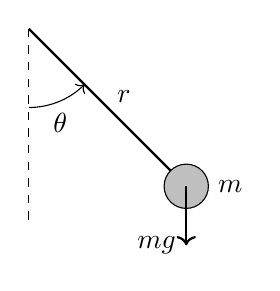
\begin{tikzpicture}
		\coordinate (O) at (0,0);
		\coordinate (P) at (2,-2);
		\draw[dashed] (O) -- ++(0,-2.5);
		
		\draw[thick] (O) -- (P);
		\draw[->] (O) -- node[midway, right, yshift=4] {$r$} (P);
		\filldraw[fill=gray!50] (P) circle (8pt);
		\node at (P) [right, xshift=8] {$m$};
		\draw[->, thick] (P) -- ++(0,-0.75) node[left] {$mg$};
		
		\draw[->] (0,-1) arc[start angle=-90,end angle=-45,radius=1];
		\node at (0.4,-1.2) {$\theta$};
	\end{tikzpicture}
}}
We want to find the relationship between the period, $\tau$ and $\theta,m,r$ and $g$. I.e. we want to find 
$$\tau = f(r, m, \theta, g)$$
First, lets find the dimensions of the system.
\begin{center}
	\begin{tabular}{|c|c|c|c|c|}
		\hline
		$[\tau]$ & $[r]$ & $[m]$ & $[\theta]$ & $[g]$ \\ \hline 
		$T$ & $L$ & $M$ & $1$ & $LT^{-2}$ \\ \hline
	\end{tabular}
\end{center}
\nt{$g$ is a dimensionless variable! In other words, its dimensions are $M^0L^0T^0$.\\}

The product of these varaibles takes the form:
$$
\tau^a r^b m^c \theta^d g^e
$$
and its dimensions are
$$
[\tau^a r^b m^c \theta^d g^e] = [\tau^a] [r^b] [m^c] [\theta^d] [g^e] = T^a\cd L^b \cd M^c \cd 1^d \cd L^eT^{-2e} = M^cL^{b+e}T^{a-2e}.
$$
Since we desire to solve represent a physical law, by claim 1.1.1, we know we're looking for a dimensionally homogeneous system.
\begin{align*}
	\Let M^cL^{b+e}T^{a-2e} &= M^0L^0T^0 \\
	\Then \left.\begin{array}{rcc}
		a - 2e & = & 0 \\
		b + e & = & 0 \\
		c & = & 0 
	\end{array}\right\rbrace& e = \frac{a}{2}, b = -\frac{a}{2}, d \text{ is free.}\\
\intertext{In other words, solve the linear system $A\utilde{x}=\utilde{0}$ (In other OTHER words, solve for the nullspace of $\cln(A)$.)}
	\tau^{a}r^{-\frac{a}{2}}m^0\theta^dg^{\frac{a}{2}} &= \bracks{\tau r^{-\half} g^\half}^a\theta^d \\
		&= \bracks{\tau\sqrt{\frac{g}{r}}}^a\theta^d
\intertext{By setting $(a,d)$ to $(1,0)$, and $(0,1)$, we obtain independent dimensionless products, $\Pi_1$ and $\Pi_2$.}
	\Pi_1 &= \tau\sqrt{\frac{g}{r}} \\
	\Pi_2 &= \theta
\end{align*}

\subsection*{The Buckingham $\Pi$-Theorem}
\thm{Buckingham $\Pi$-Theorem}{
	An equation is dimensionally homogeneous if and only if it can be written in the form
	$$
		f(\Pi_1, \Pi_2, \dots, \Pi_n) = 0,
	$$
	where $f$ is some function satisfying certain conditions (outside out scope) and $\braces{\Pi_1, \Pi_2, \dots, \Pi_n}$ is a complete set of dimensionless products corresponding to some mathematical model.
}

\nt{
	$\Pi_k$ is dimensionless, i.e.
	$\displaystyle
		\forall \Pi_k, [\Pi_k] = 1 
	$
}

The set $\bracks{\Pi_k}$ can be obtained by giving all solutions to a linear system of exponents for the model. We've found the complete set of dimensionless products for the pendulum problem, $\braces{\tau\sqrt{g/r}, \theta}$. Applying the Buckingham $\Pi$-theorem now, our mathematical model is of the form:
$$
	f(\Pi_1, \Pi_2) = 0 \implies f(\tau\sqrt{g/r}, \theta) = 0
$$
We further assume that from $f$ we can deduce 
\begin{gather*}
	\tau\sqrt{\frac{g}{r}} = h(\theta)\qquad \text{ by Implict Function Theorem.}
\end{gather*}
We'll describe implicit function theorem in detail later.

\nt{
	If $\Pi = \braces{\Pi_1, \Pi_2, \Pi_3}$, then $\Pi_1 = h(\Pi_1, \Pi_2)$. More generally, if $\Pi = \braces{\Pi_k\suchthat k\in\bbn,k\leq n}$, then $\Pi_1 = h\bracks{\Pi_2, \Pi_3, \dots, \Pi_n}$.
}

\subsection*{Archimedes' Law}
The famous ``Eureka!'' leaping from the bathtub one ;P\\

Archimedes' law applies to bodies immersed in a fluid. Consider a box of mass $m$, which displaces $V$ fluid, with constant density $\rho$. Suppose your class mate claims that this phenomenon is described by the equation
$$
	m\dyd[^2x]{t^2} = mg - mVg
$$
Let's verify this\dots
\begin{align*}
	\sqbracks{mVg} &= [m][V][g] \\
		&= M\cd L^3 \cd LT^{-2} \\
		&= ML^4T^{-2} \\
	\sqbracks{m\dyd[^2x]{t^2}} &= [m]\sqbracks{\dyd[^2x]{t^2}} \\
		&= MLT^{-2} \\
		&\neq [mVg]
\end{align*}
So we can conclude that this model is not dimensionally consistent.\\
Another classmate suggests the equation
$$
	m\dyd[^2x]{t^2} = mb - \rho Vg.
$$
We'll similarlly analyse this like
\begin{align*}
	\sqbracks{\rho Vg} &= [\rho][V][g] \\
		&= ML^{-3}\cd L^3 \cd LT^{-2} \\
		&= ML^1T^{-2} \\
		&= MLT^{-2} \\
\sqbracks{m\dyd[^2x]{t^2}} &= [m]\sqbracks{\dyd[^2x]{t^2}} \\
		&= MLT^{-2} \\
		&= \sqbracks{\rho Vg}
\end{align*}
Which is dimensionally consistent!\\

Let's use Buckingham $\Pi$-theorem to establish the general form any correct model must take:
\begin{gather*}
	\intertext{Consider the product $F^a\rho^bg^cV^dm^e$} 
	\begin{aligned}
		\sqbracks{F^a\rho^bg^cV^dm^e} &= (MLT^{-2})^a(ML^{-3})^b(LT^{-2})^c(L^3)^d(M)^e \\
			&= M^aL^aT^{-2a}\cd M^bL^{-3b}\cd L^cT^{-2c}\cd L^{3d}\cd M^e \\
			&= M^{a+b+e}L^{a-3b+c+3d}T^{-2a-2c} \\
		\Let M^0L^0T^0 &= M^{a+b+e}L^{a-3b+c+3d}T^{-2a-2c}
	\end{aligned} \\
	\Rightarrow\left.\begin{array}{rcc}
		a + b + e & = & 0 \\
		a - 3b + c + 3d & = & 0 \\
		-2a - 2c & = & 0
	\end{array}\right\rbrace\begin{array}{ccl}
		c & = & -a \\
		b & = & -a-e \\
		d & = & -a-e
	\end{array}\\
	\begin{aligned}
		\So F^a\rho^bg^cV^dm^e &= F^a\rho^{-a-e}g^{-a}V^{-a-e}m^e \\
			&= F^a\rho^{-a}g^{-a}V^{-a}\rho^{-e}V^{-e}m^e \\
			&= \bracks{F\rho^{-1}g^{-1}V^{-1}}^a \bracks{\rho^{-1}V^{-1}m}^e \\
			&= \bracks{\frac{F}{\rho gV}}^a \bracks{\frac{m}{\rho V}}^e \\
		\tf \Pi &= \braces{\frac{F}{\rho gV}, \frac{m}{\rho V}}.
	\end{aligned}
\end{gather*}

Now that we've deduced $\Pi$, we know that any valid physcial law must take the form:
$$
	\frac{F}{\rho gV} = h\bracks{\frac{m}{\rho V}}
$$
$$
	\implies F = \rho gV h\bracks{\frac{m}{\rho V}}
$$

\nt{
	Generally, when proceeding with the linear algebra portion of this procedure, keep in mind the power of your desired dependent variable, and try to express all other powers in terms of it. For example, in the pendulum example, and in the Archimedes' law exmaple too, we expressed the other variables in terms of $a$, because this was the power of the desired dependent variables $\tau$ and $F$, respectively. 
}

\pagebreak
\section{Lecture 3}
\subsection*{Drag Force}
Consider a sphere of radius $r$, moving through a viscous fluidd. We wish to model the drag force, $F$, dependent on the relevant variables $\eta$, the viscosity, $v$, the velocity, and $r$ the radius.
\begin{gather*}
	\intertext{Consider the product $F^a\eta^bv^cr^d$} 
	\begin{aligned}
		[F]^a[\eta]^b[v]^c[r]^d &= \bracks{MLT^{-2}}^a\bracks{ML^{-1} T^{-1}}^b\bracks{LT^{-1}}^c\bracks{L}^d \\
			&= \bracks{M^aL^aT^{-2a}}\bracks{M^bL^{-b}T^{-b}}\bracks{L^cT^{-c}}\bracks{L^d} \\
			&= M^{a+b}L^{a-b+c+d}T^{-2a-b-c} \\
		\Let M^0L^0T^0 &= M^{a+b}L^{a-b+c+d}T^{-2a-b-c}
	\end{aligned}\\
	\Rightarrow \left.\begin{array}{rcc}
		a + b & = & 0 \\
		a - b + c + d & = & 0 \\
		-2a - b - c & = & 0
	\end{array}\right\rbrace \begin{array}{ccl}
		b & = & -a \\
		c & = & -a \\
 		d & = & -a
	\end{array} \\
	\begin{aligned}
		\So F^a\eta^bv^cr^d &= F^a\eta^{-a}v^{-a}r^{-a} \\
			&= \bracks{F\eta^{-1}v^{-1}r^{-1}}^{a} \\
			&= \bracks{\frac{F}{\eta v r }}^{a} \\
		\tf \Pi &= \braces{\frac{F}{\eta v r }}
	\end{aligned}
\end{gather*}
So from the Buckingham $\Pi$-theorem, we know that many valid physcial law must take the form:
$$
	f\bracks{\frac{F}{\eta vr}} = 0
$$
$$
	\implies \frac{F}{\eta vr} = k
$$
In other words, $F = k\eta vr$, where $k$ is some dimensionless constant.

\nt{
	This result, that drag force is proportional to velocity is known as Stokes' Law, and in fact, the constant $k=6\pi$.
}

\subsection*{A Mixing Model}
Initially, a tank of water with $v_0$ litres has $m_0$ grams of salt dissolved in it. Brine with $n$ grams of salt per litre runs into the tank at a rate of $x$ litres per minute. The contents are constantly stirred (so you can assume that the concentration of salt is always uniform throughout the tank) and water runs out of the tank at the rate of $y$ litres per minute. Let $s(t)$ denote the amount of salt in the tank at time $t$ (measured in minutes). Determine the equation which governs the net rate of change of salt, checking that all terms are dimensionally consistent.
\begin{gather*}
	\longintertext{Let $c(t)$ denote the density of salt at time $t$.\\
	Let $v(t)$ denote the volume of water in the tank at time $t$.}
	\begin{aligned}
		\text{We have } c(t) &=\frac{s(t)}{v(t)} \\
		\text{And } v(t) &= v_0 + (x-y)t \\
		\implies c(t) &= \frac{s(t)}{v_0+(x-y)t}. \\
	\end{aligned}
	\intertext{Salt enters at a rate of $nx$ grams/minute and leaves at a rate of $yc(t)$ per minute.}
	yc(t) = \frac{ys(t)}{v_0+(x-y)t}.
	\intertext{Therefore, the net rate of change is}
	\dyd[s]{t} = nx - \frac{ys}{v_0+(x-y)t}, s(0)=m_0.
	\intertext{Now lets check the model for dimensional homogeneity!}
	\begin{aligned}
		\sqbracks{\dyd[s]{t}} &= MT^{-1} \\
		[nx] &= ML^{-3}\cd L^3T^{-1} \\
			&= MT^{-1} \\
		[v_0] &= L^3 \\
		[(x-y)t] &= L^3T^{-1}T \\
			&= L^3 \\
		\Rightarrow \sqbracks{\frac{ys}{v_0+(x-y)t}} &= \frac{ML^3T^{-1}}{L^3} \\
			&= \frac{ML^3T^{-1}}{L^3} \\
			&= MT^{-1}
		\end{aligned}\\
		\tf \sqbracks{\dyd[s]{t}} = \sqbracks{nx} = \sqbracks{\frac{ys}{v_0+(x-y)t}}
\end{gather*}
So, the system is dimensionally homogeneous.

\subsection*{Scaling}
\textbf{Question,} can we scale experiments in a laboratory to ensure that the observed effects are consistent?\\
We can use dimensionless variables, and try to preserve their values. Some examples of dimensionless variables in fluid dynamics include
\begin{gather*}
	\text{Reynold's Number,}\qquad Re = \frac{\rho lv}{\eta} \\
	\text{Froude's Number,}\qquad Fr = \frac{v}{\sqrt{gl}} \\
	\text{Mach Number,}\qquad M = \frac{v}{c}
\end{gather*}
where, $\rho$ is the fluid denisty, $l$ is the length of an object, $v$ is velocty, $\eta$ is the viscosity of the fluid, $g$ is gravitational acceleration, and $c$ is the speed of sound.

\subsection*{A Ship Model}
Suppose our model involves $Fr$, which we seek to keep fixed. \\
The true boat has hull length $l=20\text{m}$, at speed $v=10\text{ms}^{-1}$\\
We can model this with a boat of hull length $l^*=0.2m$, i.e. $l^*=l/100$. \\
What is $v^*$?
\begin{gather*}
	\begin{aligned}
		Fr &= \frac{v}{\sqrt{gl}} = \frac{v^*}{\sqrt{gl^*}} \\
		\tf v^* &= v \sqrt{\frac{gl^*}{gl}} \\
			&= v \sqrt{\frac{l^*}{l}} \\
			&= 10 \sqrt{\frac{0.2}{20}} \\
		\tf v^* &= 1 \text{ms}^{-1}
	\end{aligned}
\end{gather*}

\chapter{Week 2}
\section{Lecture 4}
\subsection*{Multivariate Limits}
\subsubsection*{Review of one-variable case}
Let $f:\rmd\to\bbr$ be a function with domain $\rmd$, an open subset of $\bbr$. For $a\in\rmd$ we say that the limit $\dps{\lim_{x\to a}f(x)}$ exists if and only if (i) the left-sided limit exist, (ii) the right-sided limit exists, and (iii) these limits equal each other, namely
$$
	\lim_{x\to a^-} f(x) = \lim_{x\to a^+} f(x).
$$
Furthermore, if the limit exists, and is equal to the value of the function at $f$, namely,
$$
	\lim_{x\to a^-} f(x) = \lim_{x\to a^+} f(x) = f(a),
$$
we say that $f$ is continuous at $a$. The precise defintion of the one variable limit its
$$
	\lim_{x\to a}f(x)=L\iff \forall\veps>0,\exists\delta>0:0<\abs{x-a}<\delta\implies\abs{f(x)-L}<\veps.
$$
\subsubsection*{The two-variable case}
When $f$ is multivariate, finding the limit is more subtle. There are more then two ways to approach a given point. Consider 
$$
	f(x,y) = \frac{x^2}{x^2+y^2},
$$
with domain $\bbr^2\setminus{(0,0)}$.
We could approach this limit along the line $y=0$. If $x\neq0$,
\begin{gather*}
	f(x,0) = \frac{x^2}{x^2 + 0} = 1, \\
	\Then \lim_{x\to0} f(x,0) = \lim_{x\to0} 1 = 1
\end{gather*}
Suppose next we approach the limit along the line $x=0$, if $y\neq0$,
\begin{gather*}
	f(0,y) = \frac{0^2}{0^2 + y^2} = 0, \\
	\Then \lim_{y\to0} f(0,y) = \lim_{y\to0} 0 = 0.
\end{gather*}
Since we've approached the same point with two different paths, but found different limits,
$$
	\lim_{x\to0} f(x,0) \neq \lim_{y\to0} f(0,y),
$$
we can conclude that
$$
	\lim_{(x,y)\to(0,0)}f(x,y) \text{ does no exist.}
$$
For the limit $\dps{\lim_{(x,y)\to(a,b)} f(x,y)}$ to exist, it is necessary that \textit{every} path in $\rmd$ approaching $(a,b)$ gives the same limiting value. This presents us with a simple test for determining if a limit does not exist.

\ex{Test for showing no limit exists}{
	$$
		\text{If}\left\lbrace\begin{array}{rl}
			f(x,y)\to L_1 & \text{as } (x,y) \to (a,b) \text{ along the path } C_1\in\rmd \\
			f(x,y)\to L_2 & \text{as } (x,y) \to (a,b) \text{ along the path } C_2\in\rmd 
		\end{array}\right.
	$$
	such that $L_1\neq L_2$ then the limit $\dps{\lim_{(x,y)\to(0,0)}f(x)}$ does not exist.
}
\nt{
	The above notation is somewhat deficient and perhaps one shoule write
	$$
		\lim_{(x,y)\to_\rmd(a,b)}f(x,y)
	$$
	to indicate that only paths in $\rmd$ terminating at $(a,b)$ (which itself may or may not be in $\rmd$) are considered.
}
\qs{}{
	Let $\rmd=\bbr^2\setminus{(0,0)}$ and $f:\rmd\to\bbr$ be given by $\dps{f(x,y)\frac{x^2-y^2}{x^2+y^2}.}$ Show that the limit $\dps{\lim_{(x,y)\to(0,0)}f(x)}$ does not exist.
}
\sol Consider the path $C_1\in\rmd,y=0$ \\ If $x\neq0$,
\begin{gather*}
	f(x,0) = \frac{x^2}{x^2} = 1. \\
	\lim_{x\to0}f(x,0) = \lim_{x\to0}1 = 1.
	\longintertext{Consider the path $C_2\in\rmd,x=0$\\If $y\neq0,$}
	f(0,y) = \frac{-y^2}{y^2} = -1. \\
	\lim_{y\to0}f(0,y) = \lim_{y\to0}-1 = -1 \neq \lim_{x\to0}f(x,0). \\
	\intertext{Therefore, the limit $\dps{\lim_{(x,y)\to(0,0)}f(x,y)}$ does not exist.}
\end{gather*}

\qs{}{
	With the same $\rmd$ as the previous question, consider $\dps{f(x,y)=\frac{xy}{x^2+y^2}}$. Show that the limit $\dps{\lim_{(x,y)\to(0,0)}f(x,y)}$ does not exist.
}
\sol Consider the path $C_1\in\rmd,y=0$ \\ If $x\neq0$,
\begin{gather*}
	f(x,0) = 0 \implies \lim_{x\to0} f(x,0) = 0 \\
	\longintertext{Consider the path $c_2\in\rmd,x=0$\\ If $y\neq0$,}
	f(0,y) = 0 \implies \lim_{y\to0} f(0,y) = 0 \\
	\longintertext{Huh\dots I really thought that would work\dots\\Well, ok, Let's consider the path $C_3\in\rmd,x=y$\\ If $x\neq0$,}
	f(x,x) = \frac{x^2}{x^2+x^2} = \frac{1}{2} \implies \lim_{x\to0} f(x,x) = \frac{1}{2}.
	\intertext{Since this limit is different from the other two, we can conclude that the limit $\dps{\lim_{(x,y)\to(0,0)}f(x,y)}$ does not exist.}
\end{gather*}
\nt{
	We can look at finitely many paths, and easily show that a limit doesn't exisit, if two paths terminating at the same point have different limiting values. But, there are infinitely many paths in $\bbr^2$ which terminate at the point $(a,b)$. This raises the question, how can we prove a limit exists?
}

\noindent Consider the example 
$$
	\lim_{(x,y)\to(0,0)} f(x,y) = 0, \text{ where } f(x,y) = \frac{3x^2y}{x^2 + y^2} \text{ and } \rmd=\bbr\setminus{(0,0)}.
$$
We can argue that the above limit is correct and true by utilising a change of variables, namely $$x=r\cos\theta \qquad y=r\sin\theta$$
\sol
\begin{gather*}
	\begin{aligned}
			f(x,y) &= f(r\cos\theta,r\sin\theta) \\
				&= \frac{3r^2\cos^2\theta r\sin\theta}{r^2\cos^2\theta + r^2\sin^2\theta} \\
				&= \frac{3r^3\cos^2\theta\sin\theta}{r^2\bracks{\cos^2\theta +\sin^2\theta}} \\
				&= 3r\cos^2\theta\sin\theta
			\abs{\cos\theta} &\leq 1\\ 
			\abs{\sin\theta} &\leq 1 \\
			\implies \abs{\cos^2\theta\sin\theta} &\leq 1 \\
			\implies \abs{3r\cos^2\theta\sin\theta} &\leq 3r \\
			\implies \abs{f(x,y)} &\leq 3r 
	\end{aligned} \\
	\tf \text{as } r\to0, f(x,y)\to 0
\end{gather*}
No matter what path of form $(r,\theta)$ we take, as that path approaches the point $(a,b)$, the limit of $f(x,y)$ approaches 0. So we can argue that $\dps{\lim_{(x,y)\to(0,0)}f(x,y)}$ exists and is equal to 0. With everything we've learned now, let's finally, formally, define the limit of a multivariate function.

\dfn{The Limit of a Multivariate Function}{
	Let $f$ be a function of two variables, whose domain $\rmd$ includes points arbitrarily close to $(a,b)$. Then we say that the limit of $f(x,y)$ as $(x,y)$ approaches $(a,b)$ is $L$, written
	$$
		\lim_{(x,y)\to(a,b)} f(x,y) = L,
	$$
	if
	$$
		\forall\veps>0,\exists\delta>0:0<\sqrt{\bracks{x-a}^2 + \bracks{y-b}^2}<\delta\implies \abs{f(x,y)-L}<\veps.
	$$
}

\pagebreak
\section{Lecture 5}
\subsection*{Multivariate Continuity}
\dfn{Multivariate Continuity}{
	Given a function $f:\rmd\to\bbr$, where $\rmd$ is an open subset of $\bbr^2$. Let $(a,b)\in\rmd$. Then $f(x,y)$ is continuous at $(a,b)$ If
	$$
		\lim_{(x,y)\to(0,0)}f(x,y)=f(a,b),
	$$
	ie, the limit $(x,y)\to(a,b)$ of $f(x,y)$ exists and is equal to $f(a,b)$.\\
	
	Equivalently, $f$ is continuous if 
	$$
		\forall\veps>0,\exists\delta>0: (x,y)\in\rmd\land\sqrt{(x-a)^2+(y-b)^2}<\delta\implies\abs{f(x,y)}<\veps.
	$$
}
\nt{
	An open subset is a subset which does not have boundary points. As opposed to a closed subset which has boundary points. More formally, ``open'' $=$ for every point $p\in\rmd$, there is a disc with centre $p$ that lies entirely in $\rmd$. So, if you took $p$ on the bounary, you can never find a disc which is entirely inside $\rmd$, you'll always have a little bit peaking out of it.
}
\noindent So, is 
$$
	f(x,y) = \frac{x^2 - y^2}{x^2 + y^2}, \rmd=\bbr^2\setminus{(0,0)}
$$
continuous?\\
Well, even though we already found that this limit $(x,y)\to(0,0)$ does not exist, we note that $(0,0)\notin\rmd$. Therefore, it is continuous.\\
If we amend the domain to include $(0,0)$, the function is no longer continous, because the limit $(x,y)\to(0,0)$ does not exist.

\subsection*{Limit Laws}
Suppose $\dps{\lim_{(x,y)\to(a,b)}f(x,y)}$ and $\dps{\lim_{(x,y)\to(a,b)}g(x,y)}$ exist. \\
Below, for ease of notation, $\lim$ denotes $\dps{\lim_{(x,y)\to(a,b)}}$. \\
\begin{enumerate}
	\item $\lim(f(x,y)\pm g(x,y)) = \lim f(x,y) \pm\lim g(x,y)$.
	\item $\lim cf(x,y) = c\lim f(x,y)$, where $c$ is some constant. 
	\item $\lim(f(x,y)\cd g(x,y)) = \lim f(x,y) \cd \lim g(x,y)$.
	\item $\dps{\lim\frac{f(x,y)}{g(x,y)} = \frac{\lim f(x,y)}{\lim g(x,y)}}$, if $\lim g(x,y)\neq 0$.
\end{enumerate}

\pagebreak
\section{Lecture 6}
\subsection*{Partial Derivatives}
\subsubsection*{Slope in the x-direction}
Consider the surface $z=f(x,y)=1-x^2-y^2$, and the point $P=(1,-1,-1)$. Holding $y$ constant, we can we can find a cross section of the surface at that point.
$$
	\Let g(x) = f(x,-1)=1-x^2-1 = -x^2
$$
We can find the slope tangent of the surface $z$ at the point $P$, in the x-direction, by differentiating $g(x)$,
$$
	g'(x) = -2x \implies g'(1) = -2
$$

\subsubsection*{Slope in the y-direction}
We can follow a similar procedure by holding $x$ constant, and generating the y-direction cross section of the surface $z$
$$
	\Let h(y) = f(1,y) = 1-1-y^2 = -y^2
$$
Now, we can evaluate the y-direction slope of the tanget of the surface $z$ at the point $P$ by taking the derivative of $h(x)$, namely
$$
	h'(x) = -2y \implies h'(-1) = 2.
$$

\subsubsection*{Another example}
Given $f(x,y)=xy^3 + x^2$, find $f_x(1,2)$ and $f_y(1,2)$.
\begin{gather*}
	\begin{aligned}
		f(x,y) &= xy^3 + x^2 \\
		\tf f_x(x,y) &= y^3 + 2x \\
		\implies f_x(1,2) &= 8 + 2 = 10 \\
		\tf f_y(x,y) &= 3xy^2 + 0 = 3xy^2 \\
		\implies f_y(1,2) &= 3\cd1\cd4 = 12 
	\end{aligned}
\end{gather*}
Nothing scary :)

\subsubsection*{Partial derivative for $f(x,y,z)$}
Consider the volume of a box, $V(x,y,z) = xyz$. If $x$ changes by an an amount, say $\Delta x$, the volume will change by some amount, $\Delta V$. One can visualise the change in volume, by imagine a box being concatonated to the original box, with width $\Delta x$, height $y$, and depth $z$. Therefore $\Delta V = yz\Delta x$. This leads us to see that
$$
	\frac{\Delta V}{\Delta x} = yz.
$$
Now, letting $\Delta x\to 0$, we can find $\dps{\frac{\partial V}{\partial x} = yz}$.\\
With partial derivatives, only one of the independent variables is allowed to change; all other variables are held constant.
$$
	\frac{\partial V}{\partial x} = \lim_{\Delta x \to 0} \frac{V(x+\Delta x, y, z) - V(x, y, z)}{\Delta x}
$$

\subsubsection*{Higher order derivatives}
\begin{multicols}{2}
	\noindent
	\begin{gather*}
		f_{xx} = \Del{2}{f}{x} \\
		f_{yy} = \Del{2}{f}{y} \\
		f_{xy} = \del{^2f}{x\partial y} = \del{}{y}\bracks{\del{f}{x}}\\
		f_{yx} = \del{^2f}{y\partial x} = \del{}{x}\bracks{\del{f}{y}}\\
	\end{gather*}
\end{multicols}
\thm{Clairaut's Theorem}{
	Suppose $f$ is defined on a disk $D$ that contains the point $(a,b)$. If the functions $f_{xy}$ and $f_{yx}$ are both continuous, then $f_{xy}(a,b) = f_{yx}(a,b)$.
}
\noindent By extension, if $f_{xy}$ and $f_{yx}$ are both continuous everywhere, then $f_{xy} = f_{yx}$.
\qs{}{
	Find all the first and second order derivatives of $f(x,y) = x\sin y + y\cos x$ and show that $f_{xy} = f_{yx}$.
}
\sol
\begin{gather*}
	\begin{aligned}
		f_x(x,y) &= \sin y - y\sin x \\
		f_y(x,y) &= x\cos y + \cos x \\
		f_{xx}(x,y)  &= -y\cos x \\
		f_{yy}(x,y) &= -x\sin y \\
		f_{xy}(x,y) &= \del{f_x}{y} \\
			&= \cos y - \sin x \\
		f_{yx}(x,y) &= \del{f_y}{x} \\
			&= 	\cos y - \sin x \\
		\tf f_{xy} &= f_{yx} 
	\end{aligned}
\end{gather*}

\noindent An unexpected feature of multivariate calculus is the possiblity that the for some point $P$, the partial derivatives of a function may be well defined, and yet, the function is not continuous at $P$. This is opposed to the one dimensional case, where we (na\"ively), assert that continuity $\implies$ differentiability. Consider 
$$
	f(x,y) = \left\lbrace\begin{array}{ll}
		\dfrac{xy}{x^2+y^2} & \text{for } (x,y)\neq(0,0) \\
		0 & \text{for } (x,y) = (0,0)
	\end{array}\right.
$$
The derivatives at $(0,0)$ are well defined:
$$
	\del{f}{x} = \frac{y^3 - x^2y}{(x^2+y^2)^2} \implies \del{f}{x}(0,0) = \lim_{h\to0} \frac{f(h, 0) - f(0,0)}{h} = \lim_{h\to 0} \frac{0 - 0}{h} = 0
$$
($\dps{\del{f}{y}}$ is defined and equal to $\dps{\del{f}{x}}$, because the function is symmetric, note that x and y can be simply interchanged in the function definition.)\\
Here, we have a function, whose derivatives are defined at a point $P$, and yet, is discontinuous at $P$.\\
When dealing with multivariate functions, existent derivatives are insufficient for determining differentiability.

\chapter{Week 3}
\section{Lecture 7}
\subsection*{The Tangent Plane}
Recall the one dimensional case, for a function $y=f(x)$, and a point $(a, f(a))$, the tangent line is given by
$$
	y_\top = f(a) + f'(a)(x-a)
$$
and can be derived by considering
\begin{gather*}
	y_\top = mx + c \\
	x = a\qquad y = f(a)\qquad m = f'(a) \\
	\tf f(a) = f'(a)a + c \\
	\tf c = f(a) - f'(a)a \\
	\tf y_\top = f'(a)x + f(a) - f'(a)a \\
	\tf y_\top = f(a) + f'(a)(x-a) 
\end{gather*}
Let's derive the vector equation for of a tangent line, consider the vector
$$
	\ut{r}(x) = (x, f(x)),
$$
and another vector which is some $\Delta x$ away from $\ut{r}$,
$$
	\ut{r}(x+\Delta x) = (x + \Delta x, f(x+\Delta x)).
$$
Now consider $\ut{r}(x+\Delta x) - \ut{r}(x) / \Delta x$. As we allow $\Delta x$ to go to 0, $\ut{r}(x+\Delta x) - \ut{r}(x)$ is going to approach the tangent line, of $f(x)$ at the point $(x,f(x))$.
$$
	\lim_{\Delta x\to 0}\frac{\ut{r}(x+\Delta x) - \ut{r}(x)}{\Delta x} = \lim_{\Delta x\to 0} \begin{pmatrix}
		\dfrac{x + \Delta x - x}{\Delta x} \\
		\dfrac{f(x+\Delta x) - f(x)}{\Delta x}
	\end{pmatrix} = \begin{pmatrix}
		1 \\ f'(x)
	\end{pmatrix}
$$
Therefore, the tangent vector, $\ut{r}_\top$ is $(1, f(x))$. Points on lying on the tangent, are 
$$
	\begin{pmatrix}
		x \\ y
	\end{pmatrix}
	=
	\begin{pmatrix}
		x_0 \\ y_0
	\end{pmatrix}
	+ 
	\lm \begin{pmatrix}
		1 \\ f'(x_0)
	\end{pmatrix},
$$
where $(x,y)$ is the point on the line, $(x_0, y_0)$ are the inital conditions, namely, the point lying on $f(x)$, and $\lambda$ is some real number. We went to all this effort, because the tangential plane of a 3D surface, is analogous to the tangential lin on a 2D curve.

\subsubsection*{Equation for the tagent plane}
On a surface $z=f(x,y)$, at the point $(a,b,f(a,b))$, the tangent plane is given by
$$
	\boxed{z_\top = f(a,b) + f_x(a,b)(x-a) + f_y(a,b)(y-b)}
$$
This is analogous to the 2D case. We follow this by defining the plane as a vector
$$
	\boxed{\ut{r}_\top = (r_1,r_2,r_3) = (a,b,f(a,b)) + \lm(1, 0, f_x(a,b)) + \mu(0, 1, f_y(a,b)),}
$$
where $\lm=x-a$ and $\mu=y-b$.\\

\noindent I like to think of it like this:
$$
	\ut{r}_x = (1, 0, f_x(a,b))\qquad \ut{r}_y = (1, 0, f_y(a,b))
$$
are linearly independent vectors. The $\Span\braces{\ut{r}_x, \ut{r}_y}$ \textit{is} the tangent plane. $\lm,\mu\in\bbr$ lets us take any linear combination of these planar basis vectors. This new vector, therefore, will lie on the tangent plane. 

\ex{Tangent Plane}{
	Find the tangent plane to the surface $z=1-x^2-y^2$ at the point $P=(1,-1,-1)$.
	\begin{gather*}
		\begin{aligned}
			f(x,y) &= 1 - x^2 - y^2 \implies f(1,-1) = -1 \\
			f_x(x,y) &= -2x \implies f_x(1,-1) = -2 \\
			f_y(x,y) &= -2y \implies f_y(1,-1) = 2 \\
			\tf z_\top &= -1 - 2(x-1) + 2(y+1) \\
				&= -1 -2x +2 +2y + 2 \\
				&= 3 - 2x + 2y 
		\end{aligned}
		\intertext{Alternatively\dots}
		\ut{r}_\top
		= 
		\begin{pmatrix}
			r_1 \\ r_2 \\ r_3
		\end{pmatrix}
		=
		\begin{pmatrix}
			1 \\ -1 \\ -1
		\end{pmatrix}
		+ 
		\lm\begin{pmatrix}
			1 \\ 0 \\ -2
		\end{pmatrix}
		+
		\mu\begin{pmatrix}
			0 \\ 1 \\ 2
		\end{pmatrix} 
		= 
		\begin{pmatrix}
			1 + x - 1 + 0 \\ -1 + 0 + y - 1 \\ -1 - 2x + 2 + 2y + 2
		\end{pmatrix}
		=
		\begin{pmatrix}
			x \\ y \\ 3 - 2x + 2y
		\end{pmatrix}
	\end{gather*}
}

\ex{Tangent Plane}{
	What is the plane tangent to the surface $f(x,y) = 4 - x^2 + 4x - y^2$, at $(1,1)$?
	\begin{gather*}
		\begin{aligned}
			f(1,1) &= 4 - 1 + 4 - 1 = 6 \\
			f_x(x,y) &= -2x + 4 \implies f_x(1,1) = 2 \\
			f_y(x,y) &= -2y \implies f_y(1,1) = -2 \\
			\tf z_\top(x,y) &= 6 + 2(x-1) - 2(y-1) \\
				&= 6 + 2x - 2 - 2y + 2 \\
				&= 6 + 2x - 2y
		\end{aligned}
	\intertext{Alternatively\dots}
	\ut{r}_\top 
	=
	\begin{pmatrix}
		r_1 \\ r_2 \\ r_3
	\end{pmatrix}
	=
	\begin{pmatrix}
		1 \\ 1 \\ 6
	\end{pmatrix}
	+
	\lm\begin{pmatrix}
		1 \\ 0 \\ 2
	\end{pmatrix}
	+
	\mu\begin{pmatrix}
		0 \\ 1 \\ -2
	\end{pmatrix}
	=
	\begin{pmatrix}
		1 + x - 1 + 0 \\ 1 + 0 + y - 1 \\ 6 + 2x - 2 - 2y + 2
	\end{pmatrix}
	=
	\begin{pmatrix}
		x \\ y \\ 6 + 2x - 2y
	\end{pmatrix}
	\end{gather*}
}

\subsubsection*{Smoothness}
A surface, $z = f(x,y)$ is smooth at a point $(a,b)$ if $f$, $f_x$ and $f_y$ are all continuous at $(a,b)$. Informally, as you zoom more and more into $(a,b)$, it looks more and more like a flat plane.\\
One way to observe this is looking at contours. As you zoom into a smooth function, the contours will straighten out. This means that, close to $(a,b)$, the surface can be approximated with a plane; in fact, approximated with the tangent plane.\\
Examples of non-smooth functions include things like Brownian motion. No matter how much you zoom into Brownian motion, it always looks rough. In fact, Brownian motion is fractal.

\pagebreak
\section{Lecture 8}
We first note, that the first order approximation of a single variable function, $f(x)$, around some point $(a, f(x))$, is a straight line tanget to that point.
$$
	f(a)\approx f(a) + f'(a)(x-a)
$$
\ex{}{
	Given $f(x)=\exp(x)$, estimate $e^{0.1}$.
	\begin{gather*}
		f(x) = \exp(x) \implies f'(x) = \exp(x) \\
		f(0) = \exp(0) = 1 \implies f'(0) = \exp(0) = 1 \\
		\tf e^{0.1} \approx f(0) + f'(0)(x-0) \\
		e^{0.1} \approx 1 + x \\
		\tf e^{0.1} \approx 1.1
	\end{gather*}
}

\subsection*{Linear Approximations for $f(x,y)$}
The corresponding linear, or first order approximation for a function $f$, of two variables, near a known point $(a,b)$, is the tangent plane centred on that point, given that $f$ is a smooth. Therefore, the approximation of $f$ at $(a,b)$ is
$$
	f(x,y)\approx f(a,b) + f_x(x,y)(x-a) + f_y(x,y)(y-b)
$$
\ex{}{
	The temperature in a region is given by $T(x) = 100 - x^2 - y^2$. Find the linear approximation to $T(x,y)$ near $(0,5)$.
	\begin{gather*}
		T(x,y) = 100 - x^2 - y^2 \implies T(0,5) = 75 \\
		T_x(x,y) = -2x \implies T_x(0,5) = 0 \\
		T_y(x,y) = -2y \implies T_y(0,5) = -10 \\
		\tf T(x,y) \approx T(0,5) + T_x(0,5)(x-0) + T_y(0,5)(y-5) \\
		T(x,y) \approx 75 + 0 + (-10)(y-5) \\
		T(x,y) \approx 125 - 10y 
	\end{gather*}
}

\ex{}{
	Find the tangent plane to $z=\exp(-x^2)\sin y$ at $(1, \pi/2)$. Use it to approximate $e^{-(0.9)^2}\sin(1.5)$.
	\begin{gather*}
		\intertext{Note: 0.9 is close to 1, and 1.5 is close to $\pi/2$.}
		f(x,y) = \exp(-x^2)\sin y \implies f(1, \pi/2) = \exp(-1) \\
		f_x(x,y) = -2x\exp(-x^2)\sin y \implies f_x(1,\pi/2) = -2\exp(-1) \\
		f_y(x,y) = \exp(-x^2)\cos y \implies f_y(1,\pi/2) = 0 \\
		z \approx f(1,\pi/2) + f_x(1,\pi/2)(x-1) + f_y(1, \pi/2)(y-\pi/2) \\
		\implies z \approx \exp(-1)(3-2x) \\
		\tf e^{-0.9^2}\sin(1.5) \approx e^{-1}\bracks{3-2\cd 0.9} \approx 0.4415
	\end{gather*}
}

\subsection*{Differentials}
If we reduce small changes $\Delta x$ and $\Delta y$ down to an infinitesimal changes, $\d x$, $\d y$, the linear approximation as
$$
	\d z = \d f = f_x(a,b)dx + f_y(a,b)dy
$$
This infinitesimal change $dz$ is called the total differential, and is definied by this equation (note the ``='', instead of an ``$\approx$'').

\begin{gather*}
	\intertext{Consider the work done by a, $W=PV$, where $P$ is pressure and $V$ is volume.}
	W(P,V) = PV \\
	W(P+\D P, V+\D V) = (P+\D P)(V+\D V) = PV + P\D V + V\D V + \D P\D V \\
	\tf \D W = P\D V + V\D V + \D P\D V \\
	\Let \d P = \D P, \text{ as }\D P\to 0, \d V = \D V, \text{ as }\D V\to 0 \\
	\tf \d W = P\d V + V\d V ( = W_P(P,V)\d P + W_V(P,V)\d V)
	\text{Note: } \D P\D V = 0
\end{gather*}

\subsection*{Estimating Error}
If the error in $x$ and $y$ is, at most$E_x$, and $E_y$, respectively, then a resaonable estimate for the worst-case error in the linear approximation of $f$ at $(a,b)$ is
$$
	|E| \approx |f_x(a,b)E_x| + |f_y(a,b)E_y|
$$

\ex{}{
	Suppose when making a metal barrel of base radius 1m, and height 2m, we allow an error of 5\% in radius and height. Estimate the worst-case error in volume.
	\begin{gather*}
		V(r,h) = \pi rh^2 \implies V_r(r,h) = 2\pi rh, V_h(r,h) = \pi r^2 \\
		\tf V(1,2) = 2\pi, V_r(1,2) = 4\pi, V_h(1,2) = \pi \\
		E_r = \frac{5}{100}r = \frac{5}{100}(1) = 0.05 \\
		E_h = \frac{5}{100}h = \frac{5}{100}(2) = 0.1 \\
		\implies |E| = |V_r(1,2)E_r| + |V_h(1,2)E_h| = \abs{4\pi \cd \frac{5}{100}} + \abs{\pi \cd \frac{10}{100}} = \frac{3\pi}{10} \\
		\implies\text{pct\% error: }\frac{|E|}{V(1,2)}\cd100 = \frac{3\pi}{10\cd2\pi}\cd100 = 15\%
		\intertext{Therefore, an estimate for the worst-case error in volume is 15\%}
	\end{gather*}
}
\nt{
	$\d V = V_r(1,2)\d r + v_h(1,2)\d h$, and $\d r = \D r = E_r$, $\d h = \D h = E_h$. \\
	$|E| = |V_r(1,2)E_r| + |V_h(1,2)E_h$. \\
	So the error in $V$ is just the differential of $V$.
}

\pagebreak
\section{Lecture 9}
\subsection*{Differentiability}
Recall that in single variable calculus, a function $f$ is differentiable at $x_0$ if there exists a number $f'(x_0)$ such that
$$
	f'(x_0) = \lim_{h\to0} \frac{f(x_0 + h) - f(x_0)}{h} 
$$
which can be rewritten as 
$$
	0 = \lim_{h\to0} \frac{f(x_0 + h) - f(x_0) - f'(x_0)h}{h}
$$
Informally, we say $f$ is differentiable at $x_0$ if, after enough zooming, we see a stright line $y(x) = f(x_0)+f'(x_0)(x-x_0)$, such that the difference $f(x_0+h) - y(x_0+h)$ goes to 0, faster then linearly in the limit as $h$ goes to 0. \\

Extending to the multivariate case, let $V\subseteq \bbr^n$. We define a function $f:V\to\bbr$ to be differentiable at $\ut{a}$ if there exists $\grad f(\ut{a})\in\bbr^n$ such that 
$$
	\lim_{\ut{h}\to \ut{0}} \frac{f(\ut{a}+\ut{h}) - f(\ut{a}) - \grad f(\ut{a})\cd\ut{h}}{||\ut{h}||} = 0
$$
Informally, we say that $f$ is differentiable at $\ut{a}$, if there is a plane $z(\ut{a}+\ut{h}) = f(\ut{a}) + \grad f(\ut{a})\cd\ut{h}$ such that $f(\ut{a}+\ut{h}) - z(\ut{a}+\ut{h})$ goes to 0 faster then linearly as $\ut{h}$ goes to $\ut{0}$. \\

As we shall see, if it is possible for a tangent plane, $z$ to exisit at the point $\ut{a}$, but for the function $f:V\to\bbr$ to not be differentiable at that point. \\

The lecturer proceeded to give us a very nice geometric interpretation of this, but I'm not going to write everything he handwrote.

\thm{}{
	If a function is differentiable at a point, then it is continuous at that point. The contrapositive of this is, if a function is not continuous at a point, then it is not differentiable at that point.
}

\thm{}{
	If all first-order partial derivatives of a function exist and are continuous at a point, then the function is differentiable at that point.
}

\chapter{Week 4}
\section{Lecture 10}
\subsection*{Gradients and Directional Derivatives}
The partial derivative $f_x$ corresponds to the slope of $f(x,y)$ in the $x$-direction. We now turn out attention to the question of slopes in arbitrary directions, such as $\ihat + 2\jhat$ or $-\jhat$. \\

Let $\ut{u}=\bracks{u_1,u_2,\dots,u_n} \in\bbr^n:||\ut{u}||=1$. The directional derivative of $f$ at the point $\ut{a}$ in the direction $\ut{u}$ be defined as:
$$
	f_{\ut{u}}(\ut{a})\equiv \lim_{t\to0} \frac{f(\ut{a} + t\ut{u}) - f(\ut{a})}{t}.
$$
It is also known as the slope of $f$ at the point $\ut{a}$ in the direction of $\ut{u}$. \\

In practice, this is quite cumbersome though. Instead, if $f$ is differentiable, we can observe that
\begin{gather*}
	\lim_{h\to0}\frac{f(\ut{a}+\ut{h}) - f(\ut{a}) - \grad f(\ut{a})\cd\ut{h}}{||\ut{h}||} = \lim_{t\to0}\frac{f(\ut{a}+t\ut{u}) - f(\ut{a}) - \grad f(\ut{a})\cd t\ut{a}}{t} = 0 \\
	\intertext{We can then write}
	\begin{align*}
		f_{\ut{u}} &= \lim_{t\to0}\frac{f(\ut{a}+t\ut{u}) - f(\ut{a})}{t} + \grad f(\ut{a})\cd \ut{u} - \grad f(\ut{a})\cd \ut{u} \\
			&= \lim_{t\to0}\frac{f(\ut{a}+t\ut{u}) - f(\ut{a}) - \grad f(\ut{a})\cd t\ut{u}}{t} + \grad f(\ut{a})\cd \ut{u}  \\
			&= \lim_{t\to0}\frac{f(\ut{a}+t\ut{u}) - f(\ut{a}) - \grad f(\ut{a})\cd t\ut{u}}{t} + \lim_{t\to0} \grad f(\ut{a})\cd \ut{u}  \\
			&= 0 + \lim_{t\to0} \grad f(\ut{a})\cd \ut{u} \\
			\Aboxed{f_{\ut{u}} &= \grad f(\ut{a})\cd \ut{u}}  
	\end{align*}
\end{gather*}
We can drop our assumption that $\ut{u}$ is a unit vector, and instead write 
$$
	f_{\ut{u}} = \grad f(\ut{a}) \cd \frac{\ut{u}}{||\ut{u}||}
$$

\subsection*{The gradient vector $\grad f$}
The gradient vector of $f$, or the gradient of $f$ is the simply the vector whose components are partial derivatives. \\

If we let $\braces{\ut{b}_1, \ut{b}_2, \dots, \ut{b}_n}$ form the canonical basis of $\bbr^n$ then,
$$
	\grad \in\bbr^n: \grad = \sum_{i=1}^{n} \ut{b_i}\del{}{x_i},
$$
where $x_i$ is the $i$th Cartesian dimension, or $i$th component of a vector in $\bbr^n$. \\

For example in two dimensions
$$
	\mathop{\text{grad}} f = \grad f = (f_x, f_y) = f_x\ihat + f_y\jhat.
$$
But this totally generalises into higher dimensions, for example, for a four variable function, $f(x,y,z,w)$,
$$
	\mathop{\text{grad}}f = \grad f = (f_x, f_y, f_z, f_w) = f_x\ihat + f_y\jhat + f_z\khat + f_w\hat{l}
$$

\ex{}{
	If $f(x,y)=x^2 - 3y^2 + 6y$, find the slope at $(1,0)$ in the direction $\ihat - 4\jhat$.
	\begin{gather*}
		\grad f = \begin{pmatrix}
			f_x \\ f_y
		\end{pmatrix} = \begin{pmatrix}
			2x \\ 6 - 6y 
		\end{pmatrix} \implies 
		\grad f(1,0) = \begin{pmatrix}
			2 \\ 6
		\end{pmatrix} \\
		\ut{u} = \begin{pmatrix}
			1 \\ -4
		\end{pmatrix} \implies
		\hat{\ut{u}} = \frac{1}{\sqrt{1^2 + 4^2}}\begin{pmatrix}
			1 \\ -4
		\end{pmatrix} = \begin{pmatrix}
			1 / \sqrt{17} \\ -4 / \sqrt{17}
		\end{pmatrix} \\
		\implies f_{(1,-4)}(1,0) = \grad f(1,0) \cd \hat{\ut{u}} = \begin{pmatrix}
			1 \\ -4
		\end{pmatrix} \cd \begin{pmatrix}
			1/\sqrt{17} \\ -4/\sqrt{17}
		\end{pmatrix} = \frac{2}{\sqrt{17}} - \frac{24}{\sqrt{17}} = \frac{-22}{\sqrt{17}}
	\end{gather*}
}

\ex{}{
	Find $f_{(1,-1)}(0,1) \text{ for } f(x,y) = x - x^2y^2 + y$
	\begin{gather*}
		\grad f = \begin{pmatrix}
			f_x \\ f_y
		\end{pmatrix} = \begin{pmatrix}
			1 - 2xy^2 \\ 1 - 2x^2y
		\end{pmatrix} \implies \grad f(0,1) = \begin{pmatrix}
			1 \\ 1
		\end{pmatrix} \\
		\ut{u} = \begin{pmatrix}
			1 \\ -1
		\end{pmatrix} \implies \hat{\ut{u}} = \frac{1}{\sqrt{1^2 + 1^2}} \begin{pmatrix}
			1 \\ -1
		\end{pmatrix}  = \begin{pmatrix}
			1 / \sqrt{2} \\ -1/\sqrt{2}
		\end{pmatrix} \\
		\implies f_{(1,-1)}(0,1) = \grad f(0,1)\cd\hat{\ut{u}} = \begin{pmatrix}
			1 \\ 1
		\end{pmatrix} \cd \begin{pmatrix}
			1/\sqrt{2} \\ -1/\sqrt{2}
		\end{pmatrix} = \frac{1}{\sqrt{2}} - \frac{1}{\sqrt{2}} = 0
	\end{gather*}
}

\subsection*{Properties of the gradient vector}
Two important properties of the gradient vector are:\\

The gradient $\grad f(a,b)$ is perpendicular to the contour line through (a,b) and points in the direction of the greatest increase of $f$. In fact, the direction and magnitude of the steepest slope at $(a,b)$ are given by $\grad f(a,b)$ and $||\grad f(a,b)||$.\\

We can understand these two facts by considering the value of $\cos\theta$ in 
$$
	f_{\ut{u}} = \grad f \cd \frac{\ut{u}}{||\ut{u}||} = ||\grad f||\cos\theta
$$
Consider $\ut{A}\cd\ut{B} = ||\ut{A}||\ ||\ut{B}||\cos\theta$
\begin{itemize}
	\item Case 1. $\theta = 0$\\ $\grad f$ and $\ut{u}$ are in the same direction.\\ $f_{\ut{u}}$ is maximised, because $\cos0 = 1$.
	\item Case 2. $\theta = \pi$\\ $\grad f$ and $\ut{u}$ are in opposite directions.\\ $f_{\ut{u}}$ is minimised, because $\cos\pi = -1$.
	\item Case 3. $\theta = \frac{k\pi}{2}$\\ $\grad f$ and $\ut{u}$ are perpendicular to each other.\\ $f_{\ut{u}}$ is 0. We can conclude $f(x,y)=C$, the value of $f$ doesn't change, as we move along the contour.
\end{itemize}

\ex{}{
	$T(x,y)=20 - 4x^2 - y^2$ describes the temperature on the surface of a metal plate. In which direction away from the point $(2,-3)$ does the temperature change most rapidly? In which directions away from the point $(2,-3)$ is the temperature not change? 

	\begin{gather*}
		T(2,-3) = 20 - 4(2)^2 - (-3)^2 = 20 - 16 - 9 = -5\\
		\intertext{The point $(2,3)$ lies on a contour line, lets find that line,}
		-5 = T(2, -3) = 20 - 4x^2 - y^2 \implies 4x^2 + y^2 = 25 \text{ an ellipses.} \\
		\implies \grad T = \begin{pmatrix}
			-8x \\ -2y
		\end{pmatrix} \implies \grad T(2,-3) = \begin{pmatrix}
			-16 \\ 6
		\end{pmatrix}
		\intertext{$\implies$At $(2,3)$, temperature is most rapidly increasing in the direction of $(-16,6)$.}
		\text{Direction of no change} = \ut{u}: \grad T\cd\ut{u} = 0 \\
		\grad T(2,-3)\cd\ut{u} = \begin{pmatrix}
			-16 \\ 6
		\end{pmatrix} \cd \begin{pmatrix}
			u_1 \\ u_2
		\end{pmatrix} = -16u_1 + 6u_2 = 0 \\
		\tf \ut{u} \in \braces{\begin{pmatrix} 6 \\ 16 \end{pmatrix}, \begin{pmatrix} -6 \\ -16 \end{pmatrix}}
	\end{gather*}
}

\section{Lecture 11}







\end{document}